\section{Introduction}
Acquisition of DWB datasets using Step and Shoot mode and overlapping bed positions result in complex datasets of PET RAW data, in relation to timing and positional information. Moreover, the addition of an initial DSB acquisition, commonly conducted for IDIF derivation purposes and providing information that allow for more complex kinetic modeling of the sampled region~\cite{Zaker2020}, increase the complexity of the PET RAW dataset. 

Suggested practices~\cite{Karakatsanis2013} and state of the art implementations~\cite{Hu2020} of DWB protocols regard the two datasets (DSB and DWB) as independent and suggest to perform independent reconstructions on each dataset. Post-reconstruction kinetic model fitting is then used to combine the TAC information over both datasets. 
Furthermore, the DWB dataset contains locations at the overlapping bed regions which are sampled two times more than central bed regions, which is the result of the overlapping sampling necessary to increase sensitivity at the bed position edges. In DWB imaging the bed overlapping results in timing information for locations that fall at the overlapping regions that combines those of adjacent bed positions. In post-reconstruction kinetic modeling, which is applied independently on each voxel TAC, suggested practices make use of modified timing information (average of two bed position timings) for voxels that fall in overlapping regions~\cite{Karakatsanis2013}. 
For dynamic reconstruction using DWB data, the independent reconstruction of bed positions and post-reconstruction overlapping of result parametric images has also been suggested~\cite{Karakatsanis2016a}, similar to practices conducted in static WB imaging~\cite{Schubert1996} but in this case extended to parametric images.
It is important to note that DWB acquired in CBM mode, although free of the need of overlapping bed acquisitions requires similar timing considerations to be taken into account for each axial location of the DWB acquisition~\cite{Karakatsanis2016b,Hu2020}.

The flexibility offered by the CASToR reconstruction platform allows for the capability of direct reconstruction of multi-bed data~\cite{Ross2004} to be expanded to dynamic reconstruction with DWB data, where the exact timing information of the dataset and all bed positions can be used within the same iterative loop. Furthermore the offered flexibility can allow for combination of the DSB and DWB datasets within one unique reconstruction loop.
In this chapter we describe how this novel DWB protocol reconstruction concept was implemented in CASToR and present results from dynamic reconstruction of DWB data of the IsotoPK study, which have also been presented in the EANM2020 conference~\cite{chalampalakis2020EANM}.
Finally we discuss the complications arising from kinetic model fitting errors in dynamic reconstruction with respect to data from DWB acquisitions. We present our work towards reduction of these errors using adaptive residual modelling for dynamic reconstruction, as presented in the IEEE-MIC2020 conference~\cite{}, which is the first time such a method has been applied on real DWB data.

\section{Methods}
\subsection{Dynamic Whole Body Datasets}
An diagram of axial position and time for a three bed position DWB protocol is shown in figure~\ref{fig_3_3:OverlapFraming}, to demonstrate the differences in timing information between central locations and locations at the bed overlapping regions. The bed locations in this example are identical to the setup used for the NHP acquisition on the Signa PET/MR described in chapter ~\ref{Chap3_1:AcquisitionOptimization}.
As it can be seen at the left diagram of figure~\ref{fig_3_3:OverlapFraming} axial positions that fall outside of the overlap region result in framing that is equal to the framing of their respective bed positions. Positions over the overlap regions, seen at the right diagram of figure~\ref{fig_3_3:OverlapFraming}, result in framing equal to that of both adjacent bed positions, which results in twice the number of frames compared to locations outside the overlap. Locations at the overlap regions are not sampled continuously from both contributing bed positions due to the interruption by the movement of the bed and system delays.  
Finally, complexity is increased when the DSB data are included, as shown in figure~\ref{fig_3_3:CompleteProtocolFraming}, with that information contributing to different locations of the DWB acquisition that might fall in overlap regions or not depending on the protocol setup. 

\begin{figure} [h!]
\centering
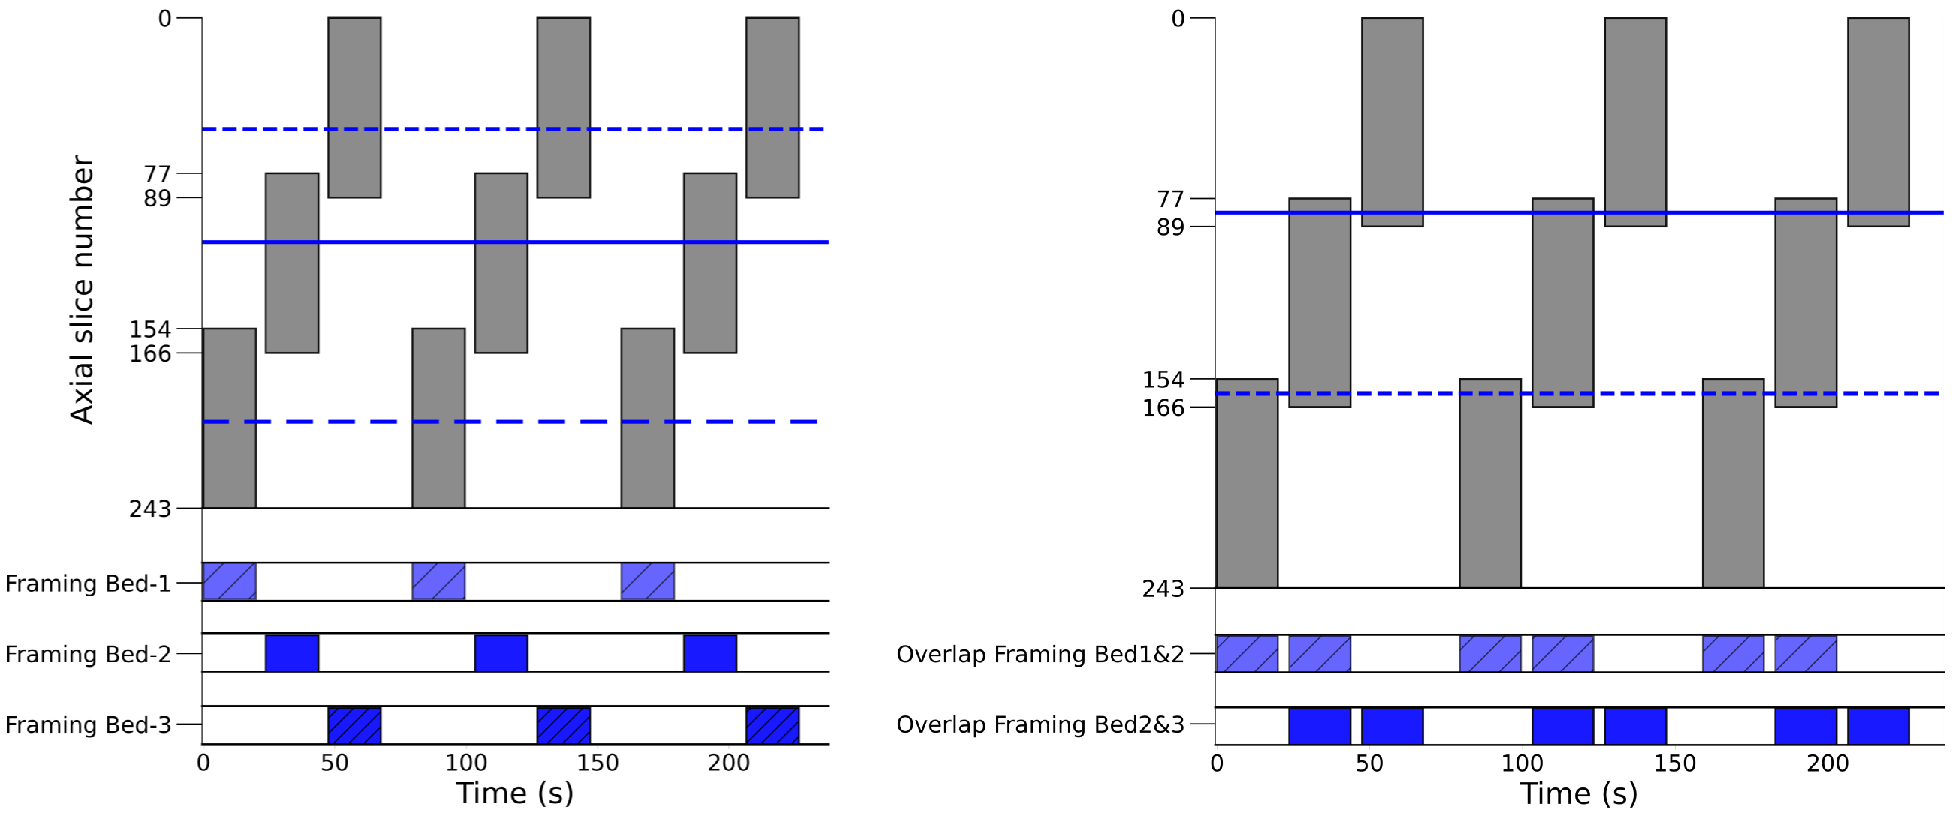
\includegraphics[scale=0.50,angle=0]{3_Results/3_3_DWB_Reconstruction/figures/OverlapTiming.pdf}
\caption{} 
\label{fig_3_3:OverlapFraming}
\end{figure} 

\begin{figure} [h!]
\centering
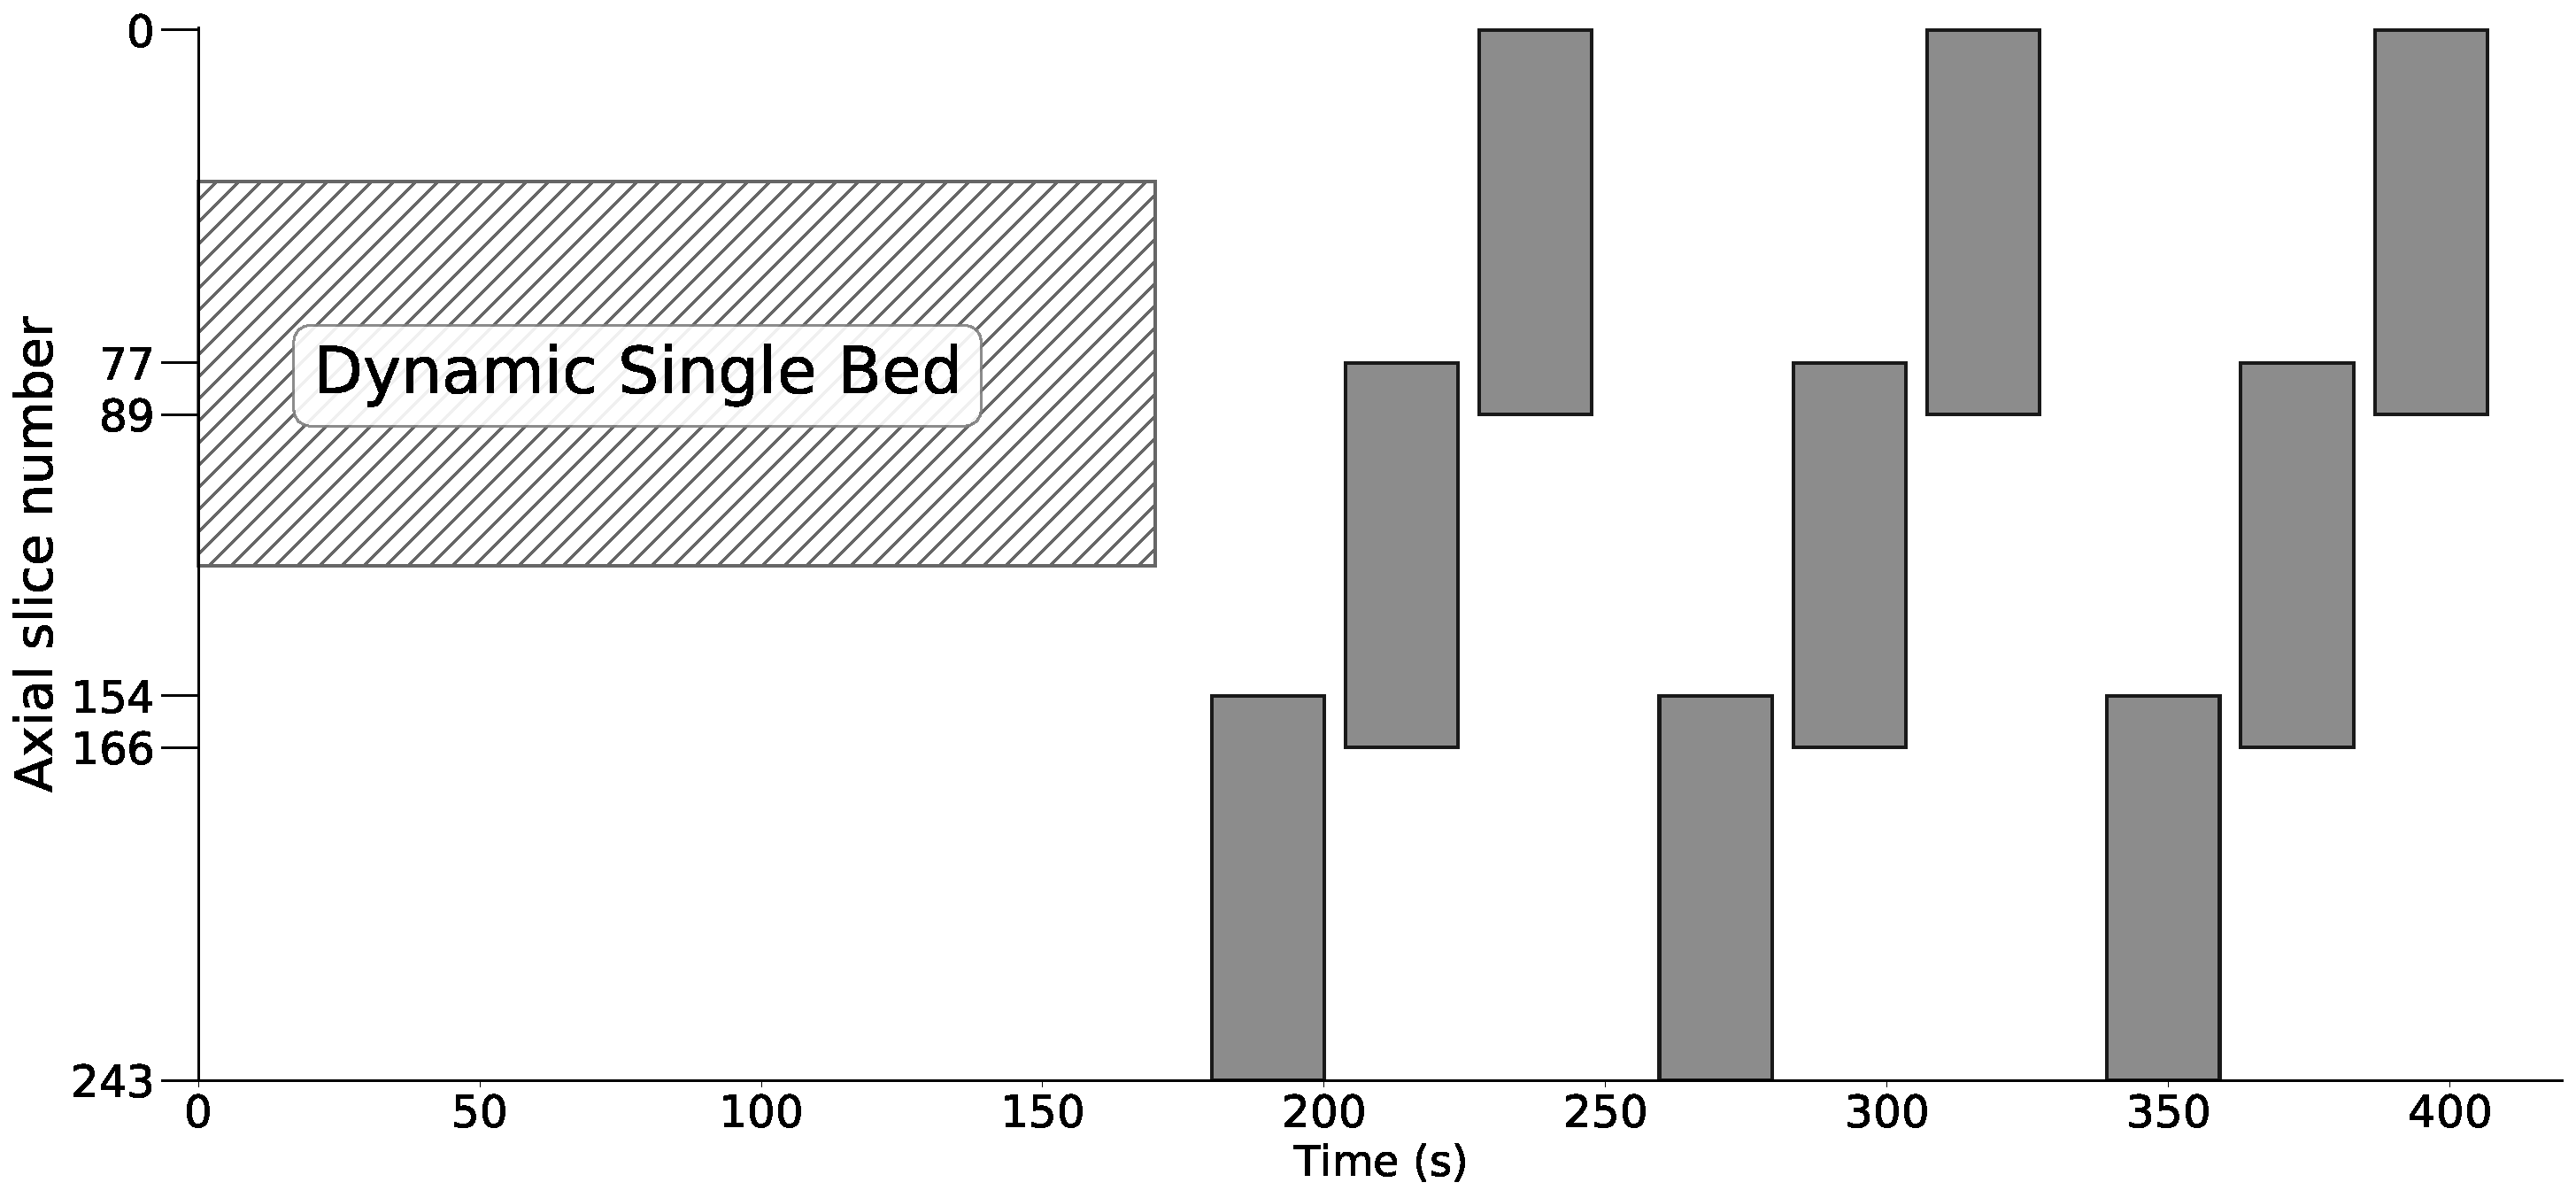
\includegraphics[scale=0.28,angle=0]{3_Results/3_3_DWB_Reconstruction/figures/CompleteProtocolTiming.pdf}
\caption{} 
\label{fig_3_3:CompleteProtocolFraming}
\end{figure} 

If considering only the DWB dataset with each individual Step and Shoot acquisition as an independent frame, the total number of frames in the DWB dataset will be defined by all the individual Step and Shoot acquisitions.% In the example presented in figure~\ref{fig_3_3:OverlapFraming} the DWB data provide nine frames. 
But not all frames need to be considered for each of the three example bed positions or for locations at the overlapping regions. 
The choice of the appropriate frames for each location, whether within or outside the overlap, can be made using an mask image that indicates which locations are sampled on each frame. This type of mask could be used for example with post-reconstruction parametric imaging, applied at each voxel to mark which frames need to be considered.

With CASToR the use of multi-bed data can be made directly within a single iterative loop, using the methodology described in section~\ref{chap2_4:MultiBedRecon}. The same framework can be extended to dynamic reconstruction of DWB datasets, using the same iterative loop. 
For linear dynamic models, dynamic reconstruction (without use of nested optimization) can be applied directly next to the system matrix, as shown in equation~\ref{eqn:4DMLEM}, within a single iterative loop over all dynamic data $y_{ti}$. 

For DWB data, incorporation of the bed offset information in the projection operation can naturally lead to direct DWB dynamic reconstruction, where the selection of the sampled time points for the location of a voxel $j$ is conducted by the projection operation. In this case the projection operation and hence the system matrix elements will depend on the frame $t$. 
This can also be conceptualised as an extension of the direct multi-bed reconstruction, described by equation~\ref{eqn2_4:MLEM_multibed}, to dynamic reconstruction where the axial offset of each bed position is incorporated in the time dependent information of the system matrix.
This provides

\begin{equation}
\theta_{pj}^{(k+1)} = \frac{\theta_{pj}^{(k)}}
{\sum_{t=1}^{n_t} B_{tp} \sum_{i=1}^{n_i} P_{tij}} 
\sum_{t=1}^{n_t} B_{tp}  \sum_{i=1}^{n_i} P_{tij} 
\frac{y_{ti}}
{\sum_{d=1}^{n_j} P_{tid} \sum_{p=1}^{n_p} B_{tp}\theta_{pj}^{(k)} + B_{ti} } \\, \\
\label{eqn:4DMLEM_Multibed}
\end{equation} 

where the set of basis functions $B$ is precomputed for all time frames of the DWB acquisition, but is effectively applied in each voxel $j$ for the time frames that are not masked by the back-projection operation $\sum_{t=1}^{n_t} \sum_{i=1}^{n_i} P_{tij}$.
It is important to note that with this unique iterative loop there is no need for additional considerations after reconstruction of the overlapping operation and regions, with the result parametric images $\boldsymbol\theta$ having dimensions of the effective FOV and having accounted for the overlap information.

Use of the same framework to perform individual frame reconstructions of DWB data is also possible, by setting the matrix $\boldsymbol{B}$ to be the identity matrix. 
An example from the use of this framework for frame reconstructions is shown in figure~\ref{fig_3_3:Macaque} for a group of three consecutive frames. The sensitivity images for the same frames, as estimated by the back-projection operation $\sum_{t=1}^{n_t} \sum_{i=1}^{n_i} P_{tij}$, are shown in figure~\ref{fig_3_3:Macaque_Sensitivity}.
The sensitivity images clearly show the sampled locations per frame and the overlapping locations for adjacent frames. 
%In this three bed acquisition a total of 243 axial slices are allocated in image space per frame, from which 89 will be sampled at each frame and bed. The overlap locations, in this case for 12 axial slices, which are sampled over consecutive frames can be identified from the frames sensitivity image. 
Individual frame reconstruction of DWB data, using this unique frame work, results directly to images of the effective FOV that account for the bed offset in image space, which can subsequently be directly used for post-reconstruction kinetic model fitting without the need for additional considerations. Additionally, for post-reconstruction kinetic model fitting, the result sensitivity frame images can be used as a mask for the applied dynamic model to identify sampled frames at each voxels location.

%
\begin{figure} [h!]
%\centering
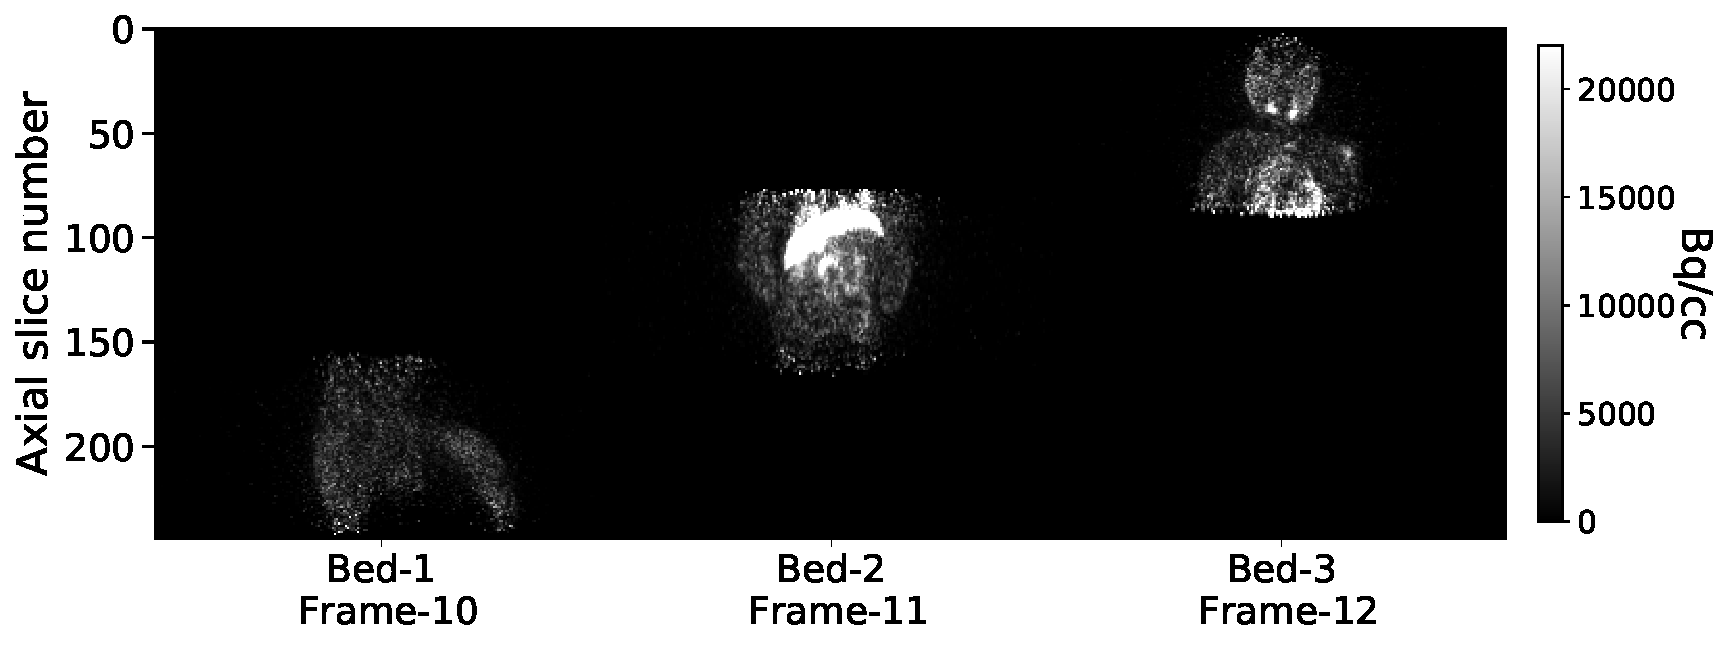
\includegraphics[scale=0.5,angle=0]{3_Results/3_3_DWB_Reconstruction/figures/Macaque_3D.pdf}
\caption{Example three frame image from a three bed positions DWB acquisition.} 
\label{fig_3_3:Macaque}
\end{figure} 
%
\begin{figure} [h!]
%\centering
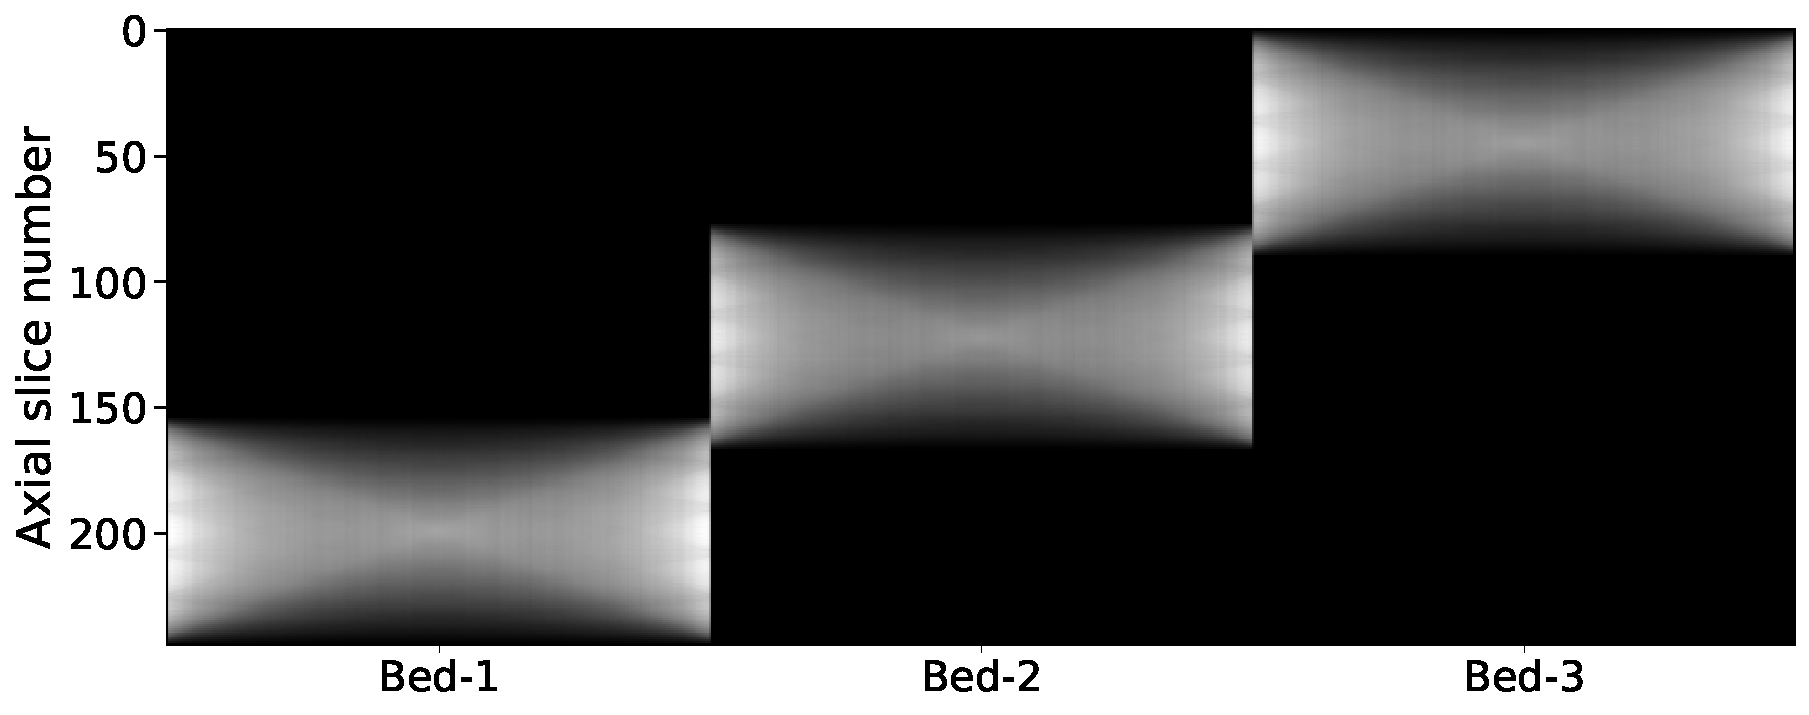
\includegraphics[scale=0.42,angle=0]{3_Results/3_3_DWB_Reconstruction/figures/Macaque_Sensitivity.pdf}
\caption{Example three frame sensitivity image from a three bed positions DWB acquisition.} 
\label{fig_3_3:Macaque_Sensitivity}
\end{figure} 
%
In addition to DWB data alone, the described methodology for direct multi-bed dynamic reconstruction allows for any sequence of the acquired bed/frames to be used within the iterative reconstruction loop. Furthermore, the use of the DSB dataset can also be included in the iterative loop, while also being sub-divided into multiple short frames.

\subsection{Dynamic reconstruction: nested optimization for DWB datasets}
As described previously, dynamic reconstruction is for practical reasons performed using the nested optimization framework, to accelerate convergence~\cite{Wang2010,Matthews2010}.
Additional considerations need to be made for use of this framework for direct multi-bed dynamic reconstruction.

The nested optimization framework decouples the tomographic update process over the raw PET data from the dynamic model fitting process on image space data. The two steps are conducted respectively with an MLEM update over the PET raw data using equation~\ref{eqn:EM_Update_image} to get an individual EM update image for each frame, followed by kinetic model fitting with optimization of the likelihood function of equation~\ref{eqn:NestedOptimization}. 

For single bed dynamic data the sensitivity term of the likelihood function over image space can be ignored, assuming that it is constant over time for each voxel, and the likelihood function can be optimised using an image based EM update over image space with equation~\ref{eqn:NestedEM}~\cite{Wang2010,Reader2014}.

In the case of DWB data and overlapping bed positions the sensitivity term has to be maintained, as its value will change with different frames for voxels in the overlapping regions.
Thus the two step process, for direct multi-bed dynamic reconstruction with nested optimization, can be written as

\begin{equation}
\label{eq3_3:NestedMultibed}
\text{}
\begin{cases}  
f_{tj}^{(EM)} = \frac{f_j(\bm\theta^{(k)})}{\sum_{i=1}^{n_i} P_{tij}} 
\sum_{i=1}^{n_i} P_{tij} 
\frac{y_{ti}}{\sum_{d=1}^{n_j} P_{tid} f_d(\bm\theta^{(k)}) + B_{ti} } \\ \\
\argmax{\bm{\theta}} 
\sum_{t=1}^{n_t} \sum_{b=1}^{n_j} \left[ \sum_{i=1}^{n_i}  P_{tib} \right]
\left[ -f_b(\bm\theta^{(k)}) + 
ln( f_b(\bm\theta^{(k)})) 
f_{tb}^{(EM)}(\bm{\theta}^{(k)})
\right] .\\
\end{cases}
\end{equation}

The tomographic update of this two-step optimization process is effectively an update over the DWB data for independent frame reconstruction, followed by an image space optimization process that now needs to consider the sensitivity $\sum_{s=1}^{n_s} \sum_{i=1}^{n_i}  P_{sib}$ of each time point $t$ in the TAC of each voxel $j$. For linear models, where before an image based MLEM algorithm was used for this image space optimization process, an weighted MLEM update can be used with the sensitivity of each time point $t$ as the weight. Alternatively, for linear and non-linear models LS based optimization algorithms can be used for models estimation with the addition of the the sensitivity value as weight.
%
\iffalse 
\begin{equation}
\theta_j^{(k+1)} = \frac{\theta_j^{(k)}}
{\sum_{p=1}^{n_p} w B_{pj}}
\sum_{p=1}^{n_p} w B_{pj} 
\frac{f_{j}^{(EM)}(\bm{\theta}^{(k)})}{\sum_{d=1}^{n_j} B_{pd}\theta_d^{(k)} } \\.
\label{eqn3_3:WeightedNestedEM}
\end{equation}
\fi
%
\subsection{Real Data}
Two DWB scans from the IsotoPK study were used for assessing direct multi-bed dynamic reconstruction methods for DWB PET imaging. Both scans were conducted on a single volunteer on a single day, without and with the use of the inhibitor (rifampicin) respectively. The volunteer scans was a male (25y) and weighted 66Kg during the examination. The two dynamic scans were conducted with injection of 141.53 MBq and 90.77 MBq of [$^{11}$C] Glyburide respectively. The first scan was conducted with 14 WB passes, with 9$\times$20, 5$\times$ s frames per bed position. The second scan included 15 WB passes, with 9$\times$20, 6$\times$ s frames per bed position. Both scans started with an 180 s DSB acquisition centered over the liver, starting at the time of injection, before the DWB acquisition. By splitting the DSB into 18x10 s frames and considering each Step and Shoot acquisition as an individual frame, the two scans resulted in a total of 88 and 93 frames respectively. 
The two scans will be refereed to as \textit{CTRL} and \textit{RIF} scans, standing for control and rifampicin. 
The planned bed positions are shown in figure~\ref{fig_3_3:IsotoPK_BedPositionsOnMR} for the DSB and DWB phase of the two scans. 

The complete \textit{CTRL} and \textit{RIF} datasets, including the DSB and DWB data, were reconstructed within the developed direct multi-bed dynamic reconstruction platform, using an OSEM algorithm with 28 subsets, with the EM nested optimization technique and 20 sub-iterations. Both datasets made use of TOF information within the reconstruction. The dynamic reconstructions were performed for DWB data, with and without the use of the initial DSB data to test extrapolation of the spectral model on early (non-sampled) frames. 
A total number of 17 spectral basis functions were used, with $\beta_1 ... \beta_{M-1}$ logarithmically spaced within the range of 3 to 0.001 $min^{-1}$, while including $\beta_0$ and $\beta_{M}$ to account for trapping and blood fraction in the data. Similarly to the simulation study, the assumption of $C_{B}$ being proportional to $C_{P}$ was used in the estimation of the basis functions.
In addition to the dynamic reconstructions, individual 3D reconstructions were performed using the same framework and OSEM algorithm with 28 subsets. As the IsotoPK study is an exploratory pharmacokinetic study, dynamic reconstructions were performed with the spectral model for temporal regularisation of frame activity estimates as well as for exploring direct estimation of $K_1$ parametric images. 

Manual arterial blood samples were taken during both scans, to derive the input function and for blood analysis (to measure the metabolites fraction and for plasma binding of the tracer). The measured input function was linearly interpolated and then used for estimation of the spectral basis functions used for reconstruction. 

\begin{figure} [h!]
\centering
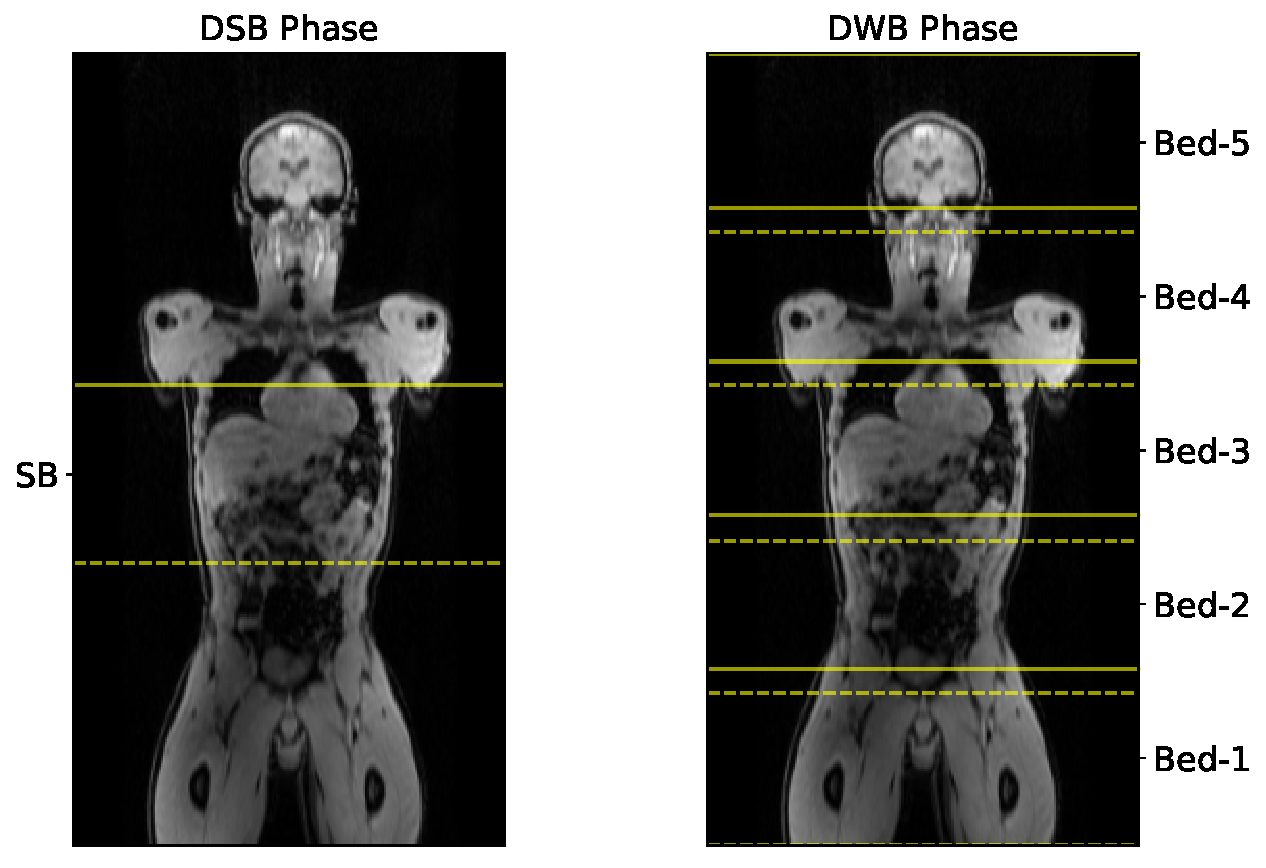
\includegraphics[scale=0.42,angle=0]{3_Results/3_3_DWB_Reconstruction/figures/3_3_IsotoPK_CTRL_PositionsOnMR.pdf}
\caption{Planned DSB and DWB bed positions on MRAC map, acquired and planned before the injection of tracer, shown with bed start (\protect\tikz[baseline]{\protect\draw[line width=0.5mm] (0,.8ex)--++(1,0) ;}) and end (\protect\tikz[baseline]{\protect\draw[line width=0.5mm,densely dashed] (0,.8ex)--++(1,0) ;}) positions.} 
\label{fig_3_3:IsotoPK_BedPositionsOnMR}
\end{figure} 

The following VOIs were manually drawn to measure statistics for validation and comparison of the reconstruction methods.
The 
\begin{table}[]
\centering
\caption{\label{tab:IsotoPK_VOIs} VOIs used for evaluation DWB evaluation.}
\begin{tabular}{lll}
\toprule
\textbf{VOI Name} & \textbf{Availability in Data}  \\
\midrule
Brain        & DWB                 \\
Myocardium & DSB \& DWB              \\
Left Ventricle (LV) & DSB \& DWB     \\
Left Kidney (Kidney$_\mathrm{L}$) & DSB \& DWB  \\
Right Kidney (Kidney$_\mathrm{R}$) & DSB \& DWB \\
Spleen & DSB \& DWB \\
Liver  & DSB \& DWB \\
Aorta & DSB \& DWB \\
Bladder & DWB \\
Leg Muscle & DWB \\
\toprule
\end{tabular}
\end{table}


\section{Results}
\subsection{Comparison between 3D and 4D spectral reconstruction on DWB data}
\Gls{mip} images of 3D reconstructions from the \textit{CTRL} scan are shown in figure~\ref{fig_3_3:IsotoPK_CTRL_DSB_3D} and figure~\ref{fig_3_3:IsotoPK_CTRL_DWB_3D}, for a late frame of the DSB acquisition and early frames of the DWB acquisition respectively. 
Similarly, \gls{mip} images of 4D spectral reconstruction of the \textit{CTRL} scan are shown in figure~\ref{fig_3_3:IsotoPK_CTRL_DSB_4D} and figure~\ref{fig_3_3:IsotoPK_CTRL_DWB_4D} for the same respective frames. 
As the spectral model is applied on the image space of the entire effective FOV, the 4D reconstruction results in frame images that are estimated from the fitted model of the entire FOV. As such, for frames within the DWB scan that are not sampled during that frame, activity estimates are interpolated from the frame data of the entire DWB scan. For the frames of the DSB scan, locations that are not sampled by the single bed acquisition have activity estimates that are extrapolated for early frames from the fitted spectral model of later frames.

\begin{figure} [h!]
\centering
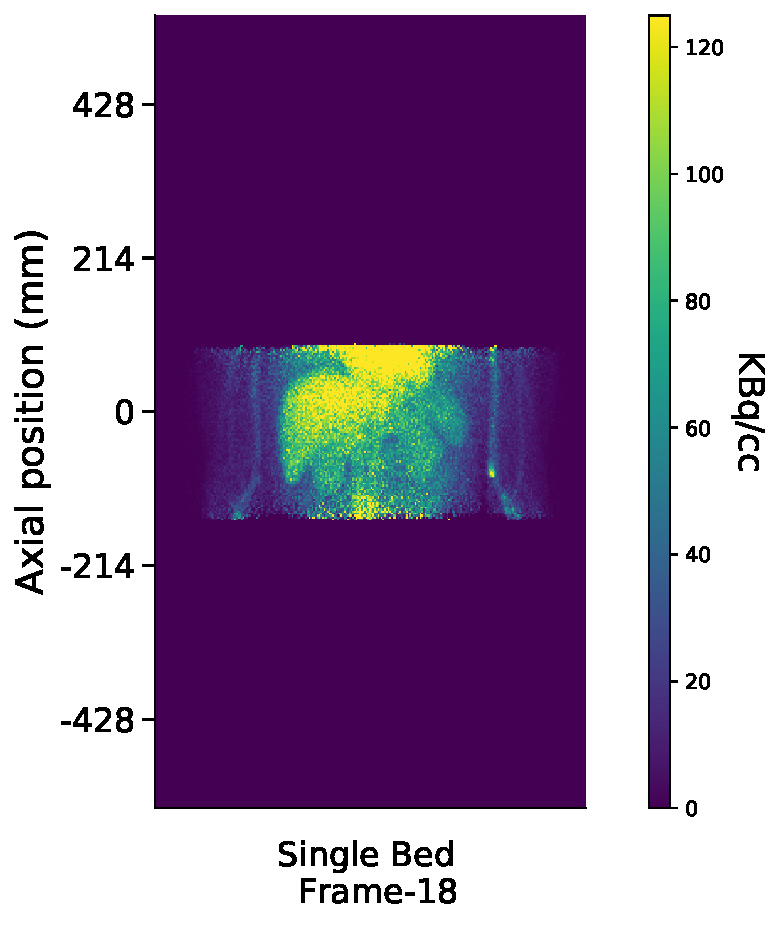
\includegraphics[scale=0.52,angle=0]{3_Results/3_3_DWB_Reconstruction/figures/3_3_IsotoPK_CTRL_DSB_3D.pdf}
\caption{MIP image of 3D reconstruction (4it28sub) of a single frame from the DSB acquisition on the \textit{CTRL} scan}
\label{fig_3_3:IsotoPK_CTRL_DSB_3D}
\end{figure} 

\begin{figure} [h!]
\centering
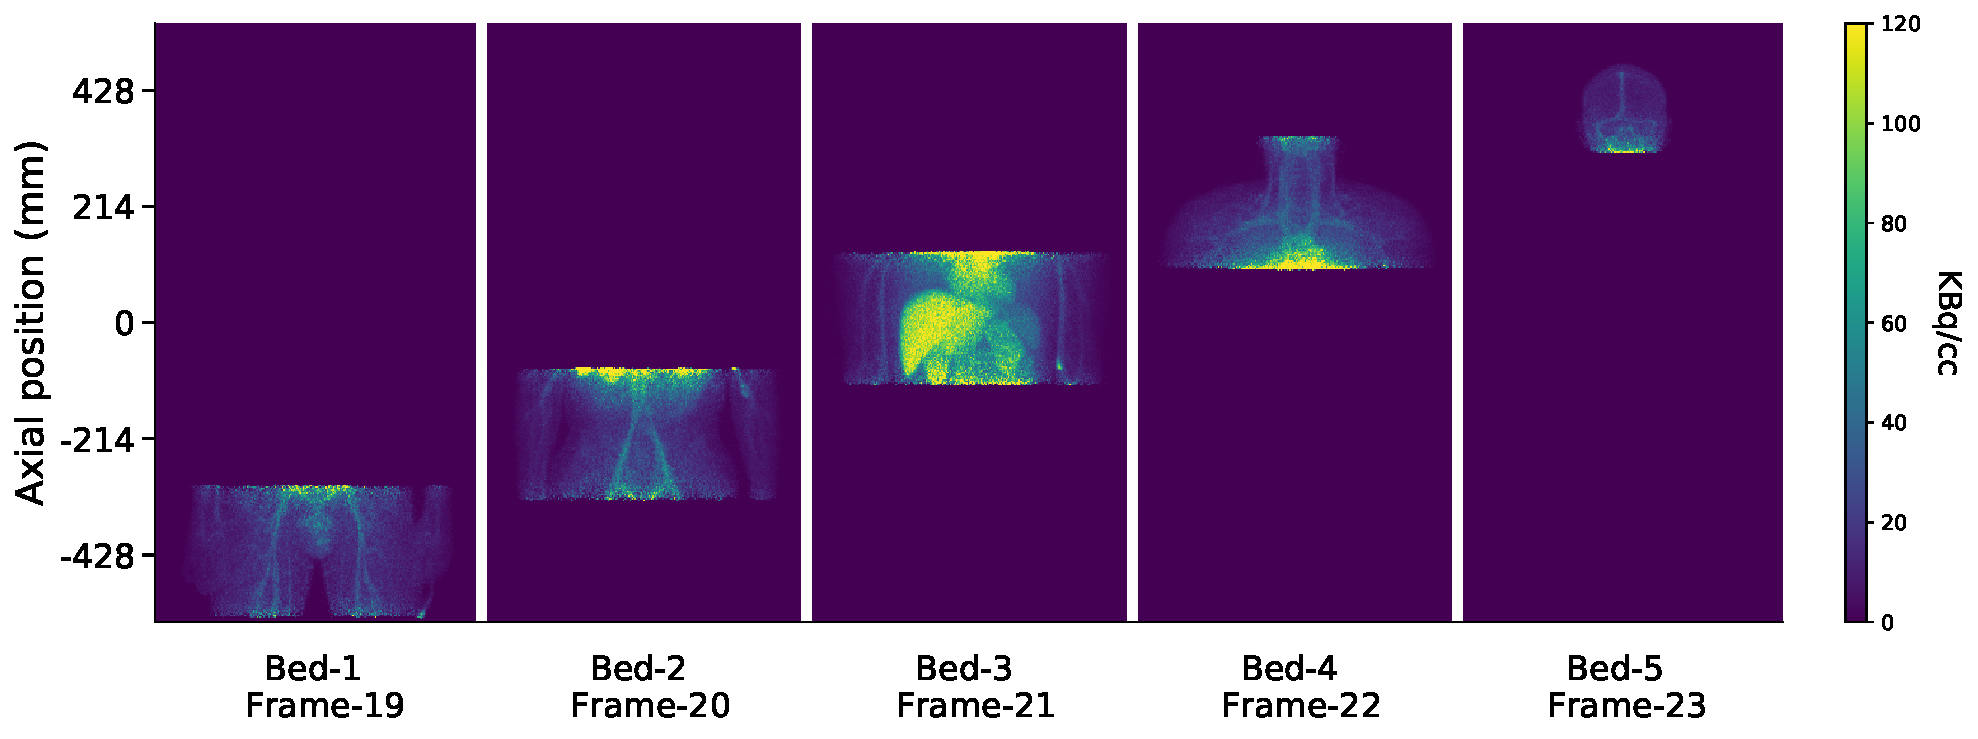
\includegraphics[scale=0.52,angle=0]{3_Results/3_3_DWB_Reconstruction/figures/3_3_IsotoPK_CTRL_DWB_3D.pdf}
\caption{MIP images of 3D reconstructions (4it28sub) of a single frame per bed position from the first whole-body pass of the DWB acquisition on the \textit{CTRL} scan.}
\label{fig_3_3:IsotoPK_CTRL_DWB_3D}
\end{figure} 

\begin{figure} [h!]
\centering
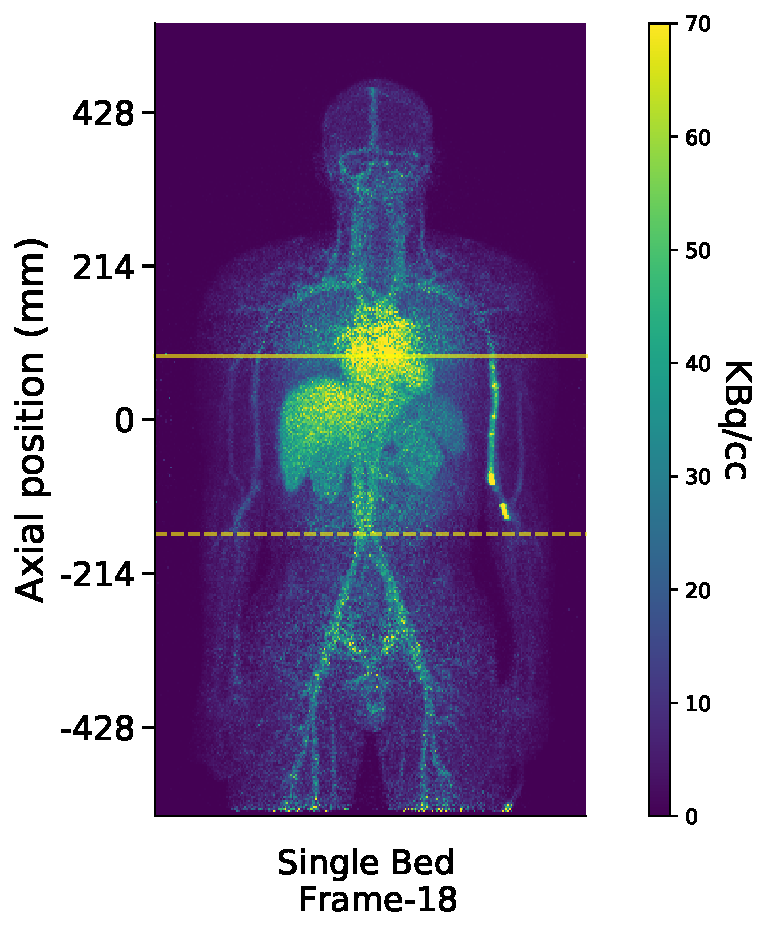
\includegraphics[scale=0.52,angle=0]{3_Results/3_3_DWB_Reconstruction/figures/3_3_IsotoPK_CTRL_DSB_4D.pdf}
\caption{MIP image of 4D reconstruction of a single frame from the DSB acquisition on the CTRL scan}
\label{fig_3_3:IsotoPK_CTRL_DSB_4D}
\end{figure} 

\begin{figure} [h!]
\centering
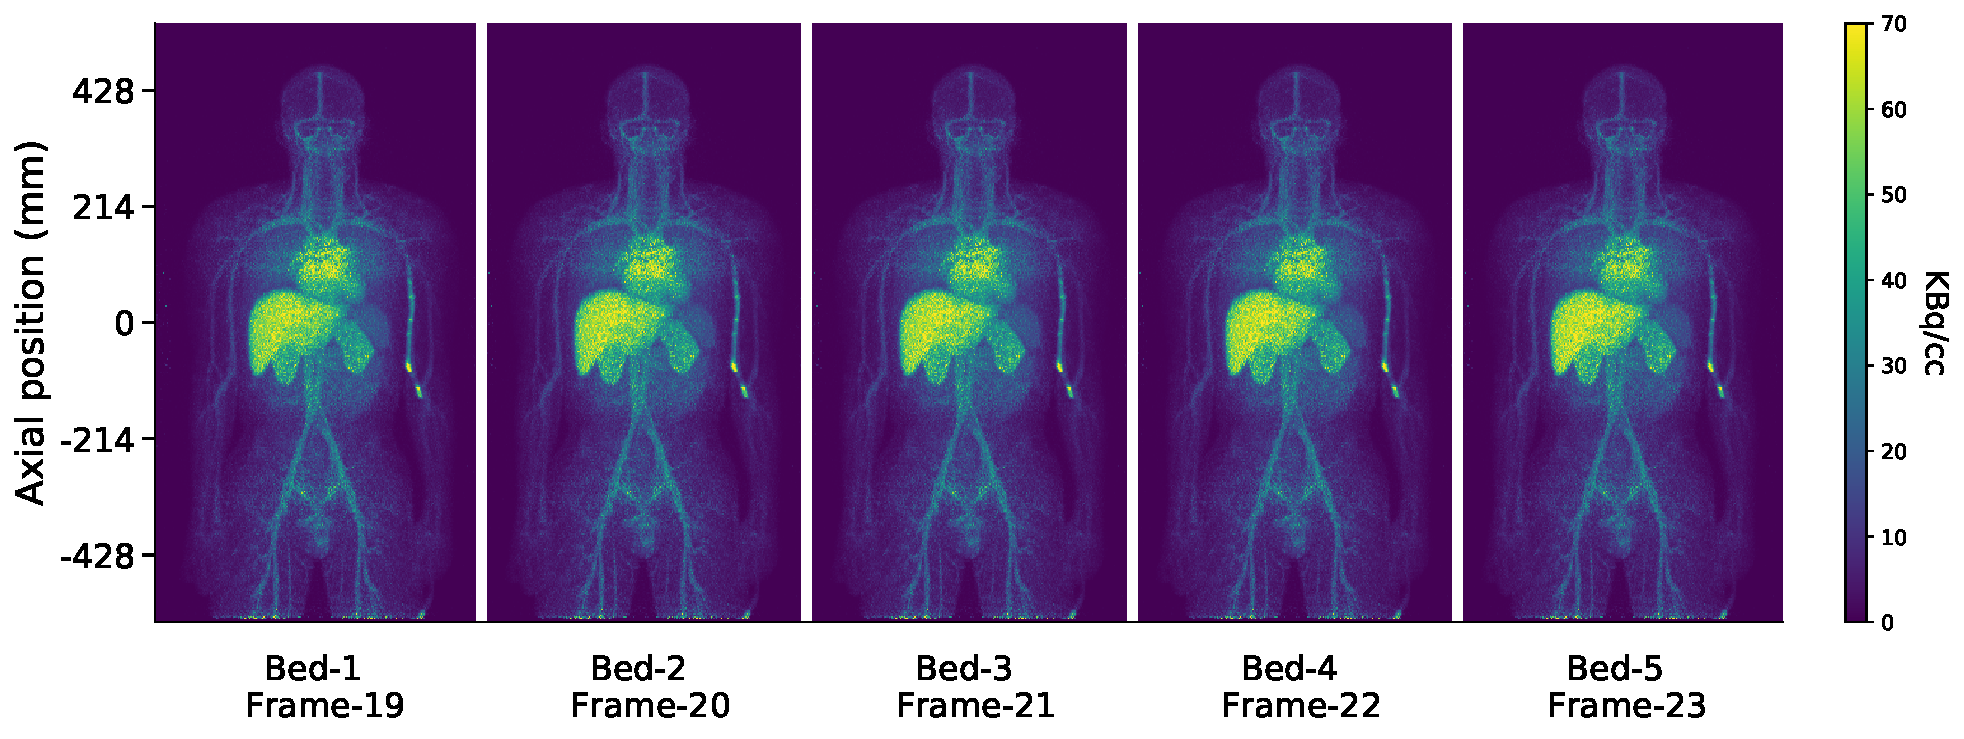
\includegraphics[scale=0.52,angle=0]{3_Results/3_3_DWB_Reconstruction/figures/3_3_IsotoPK_CTRL_DWB_4D.pdf}
\caption{MIP images of 3D reconstructions of a single frame per bed position from the first whole-body pass of the DWB acquisition on the CTRL scan.}
\label{fig_3_3:IsotoPK_CTRL_DWB_4D}
\end{figure} 

Plots of mean VOI activity against iteration, for early and late frames, over the liver and the leg muscle VOI were used to evaluate at which iteration the mean values begin to stabilise. These plots are shown in figure~\ref{fig_3_3:IsotoPK_CTRL_DWB_4D_Convergence} and figure~\ref{fig_3_3:IsotoPK_CTRL_DSB_3D_Convergence}. For 4D spectral reconstruction the evaluated mean values provided relatively stable values from the 15th iteration onwards, which was chosen for subsequent comparisons of reconstructions. For 3D reconstruction mean values did not show stable behaviour in both regions within the first 8 iterations and the 4th iteration was chosen in subsequent comparisons as a comprise between reliability of mean values and image noise.  



TACs of the evaluated VOIs are plotted in figure~\ref{fig_3_3:IsotoPK_CTRL_DWB_4D_vs_3D_Central} and~\ref{fig_3_3:IsotoPK_CTRL_DWB_4D_vs_3D_Peripheral} for VOIs sampled in both DSB and DWB acquisitions and for VOIs sampled only during the DWB acquisition respectively. In figure~\ref{fig_3_3:IsotoPK_CTRL_DWB_4D_vs_3D_Peripheral} the time point of the start of the DWB acquisition is indicated by the red dotted line.
As already mentioned, the 4D spectral reconstruction results in an activity estimate of every location of the image for every frame of the study, while 3D reconstruction results in activity estimates for the sampled frames only at each location. This is why the TACs from the 4D reconstruction of the \textit{CTRL} data show a total of 88 frame points for all VOIs and a total of 32 frame points (18 from DSB plus 14 from DWB) for central regions and only 14 frames for regions seen soley by the DWB acquisition. 

For the VOIs seen by both DSB and DWB acquisitions the TACs between 3D and 4D spectral reconstruction are in good agreement for all evaluated VOIs, as seen in~\ref{fig_3_3:IsotoPK_CTRL_DWB_4D_vs_3D_Central}. For the brain and muscle VOIs seen by the DWB acquisition only, there is a relatively good agreement with slightly overestimation in early frames of the brain region and underestimation on later frames as seen in~\ref{fig_3_3:IsotoPK_CTRL_DWB_4D_vs_3D_Peripheral}. By contrast, at the bladder VOI there is a strong mismatch of the 3D and 4D spectral reconstruction, with the 3D reconstruction showing clearly the bladder filling process and the 4D spectral reconstruction showing an increasing behaviour produced by the exponential function. 

A look into the VOI means of the spectral parametric images is given in the appendix material, where it is seen that the component of full trapping $\phi_0$ is strongly used in the bladder region, in an attempt to fit the underlying process. But any use of the input function and the decaying exponentials is not enough to fit this process. Further considerations to this issue are addressed in the the section~\ref{sub_section:residuals}. 

\begin{figure} [h!]
\centering
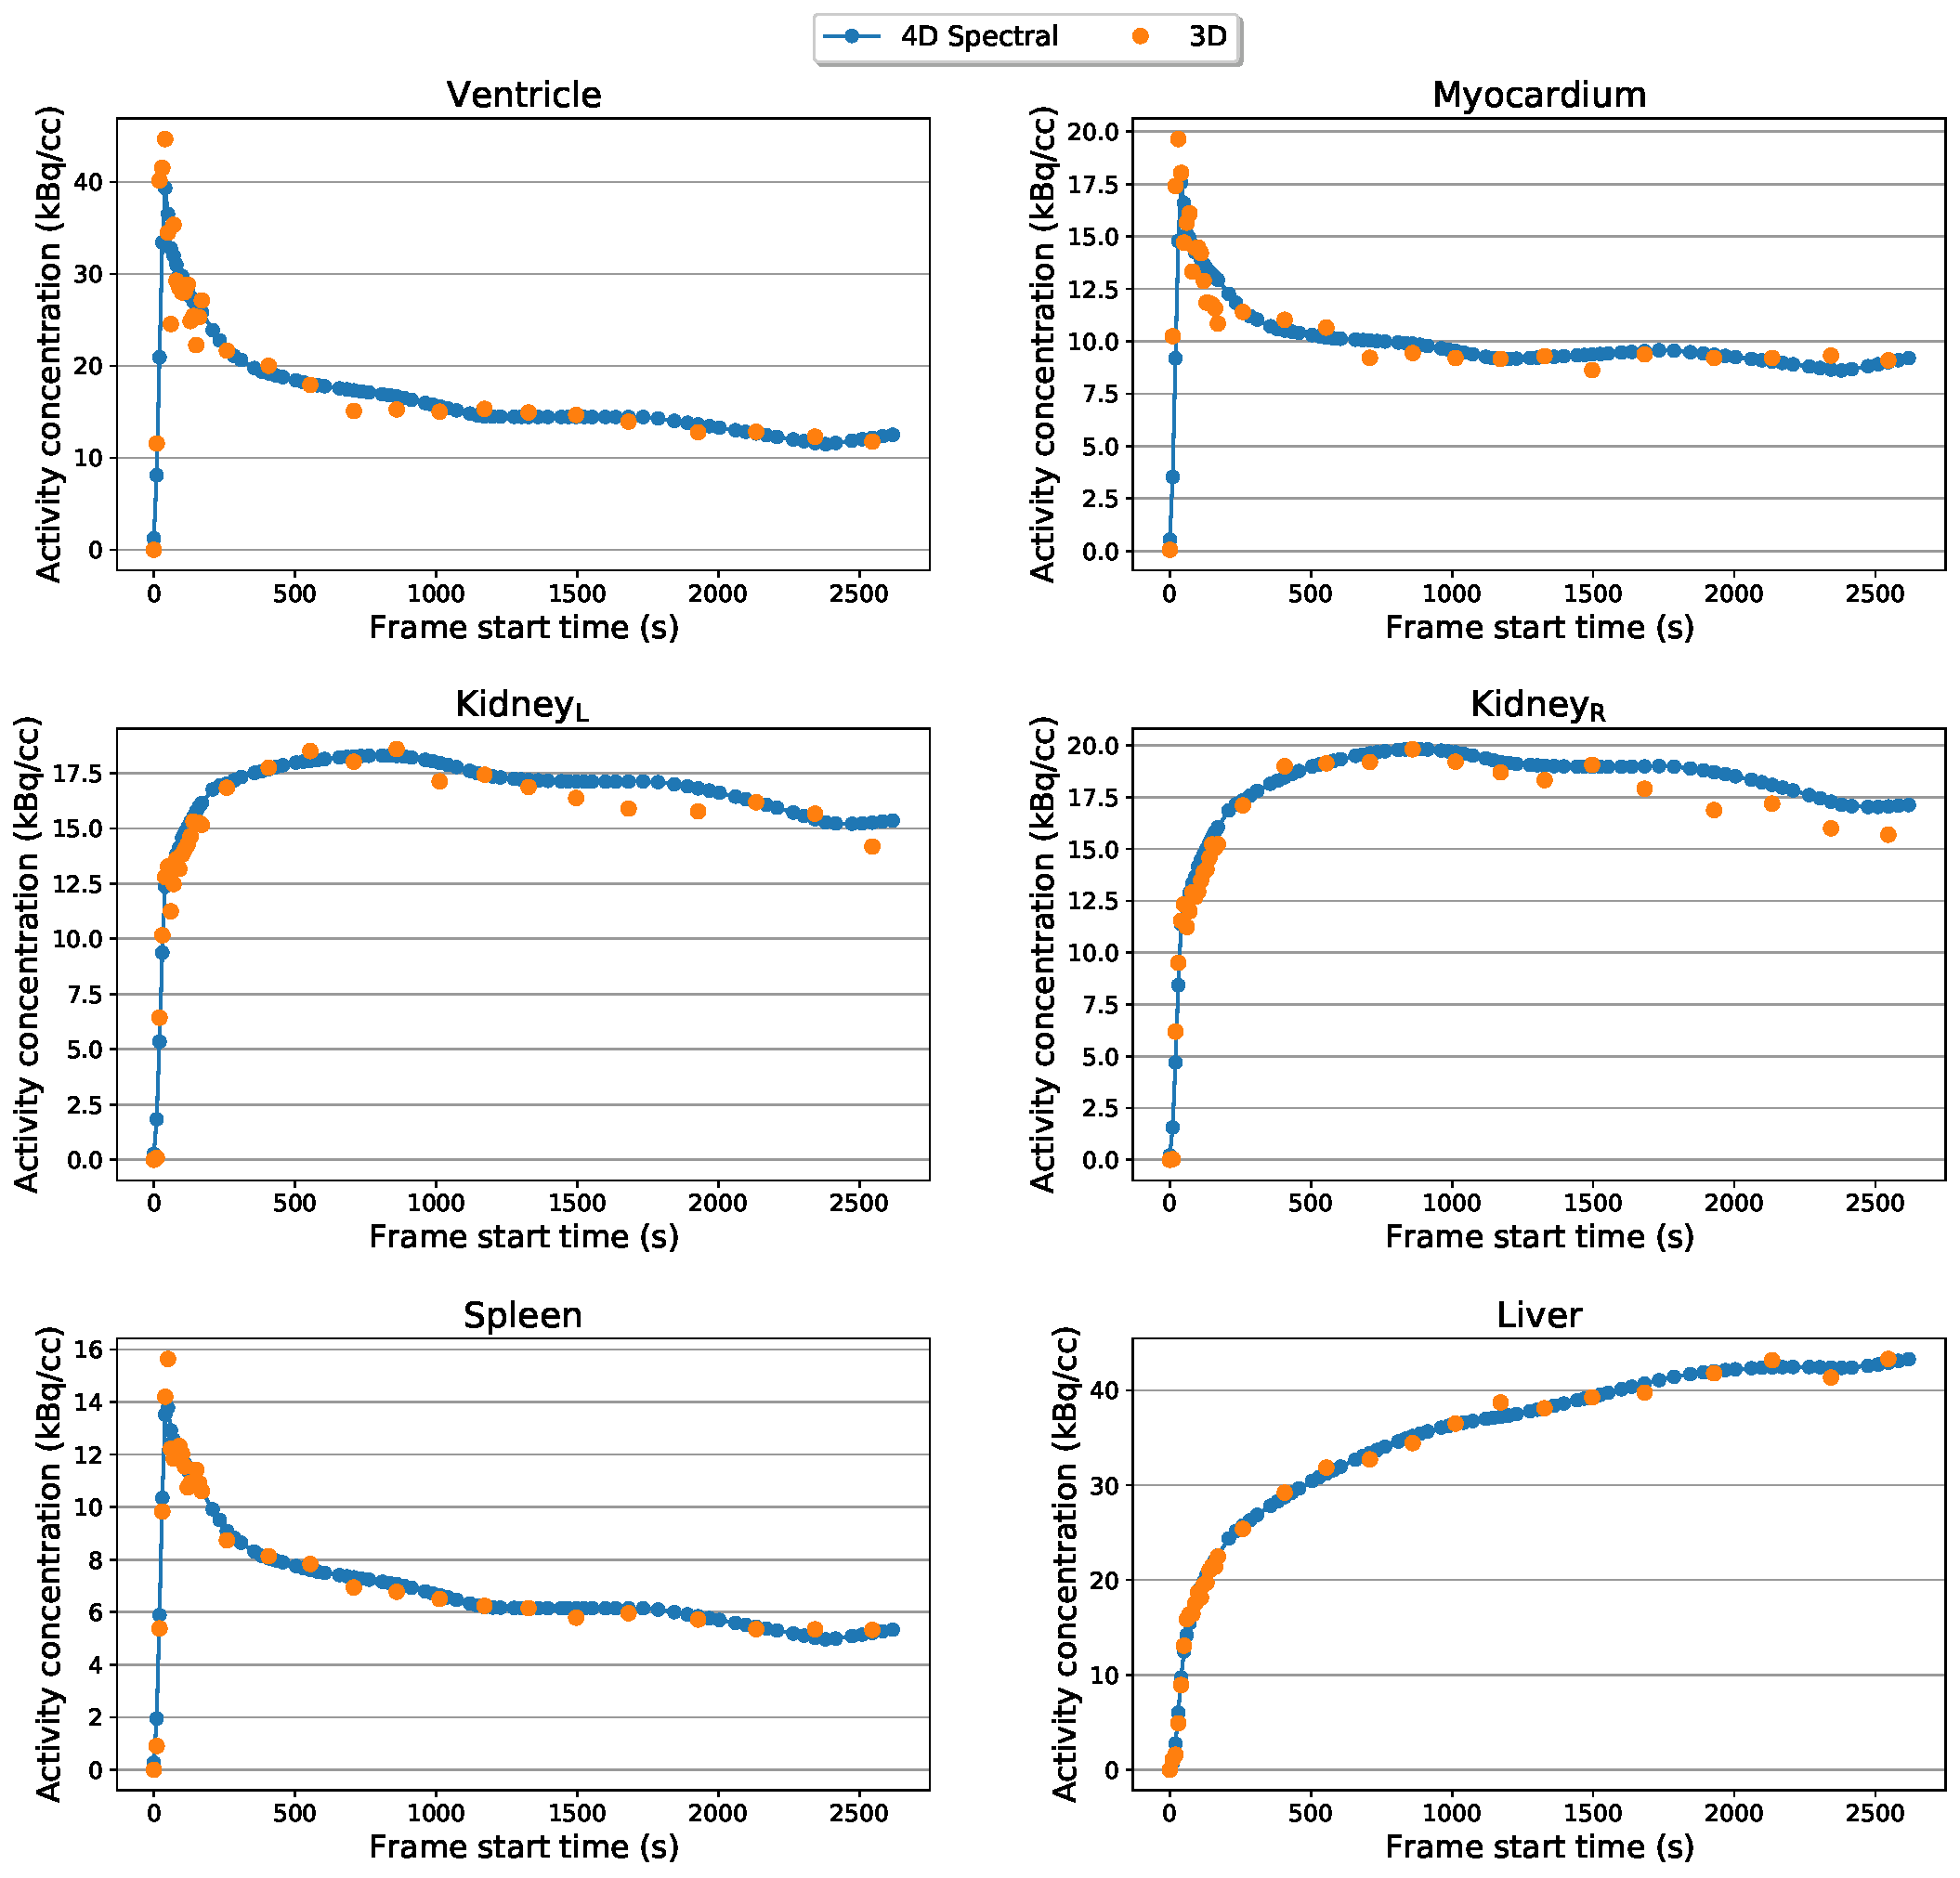
\includegraphics[scale=0.5,angle=0]{3_Results/3_3_DWB_Reconstruction/figures/3_3_IsotoPK_CTRL_DWB_3D_vs_4D_central.pdf}
\caption{VOI mean time activity curves for 3D and 4D spectral reconstruction. VOI regions shown which are included in both DSB and DWB acquisition.}
\label{fig_3_3:IsotoPK_CTRL_DWB_4D_vs_3D_Central}
\end{figure}

\begin{figure} [h!]
\centering
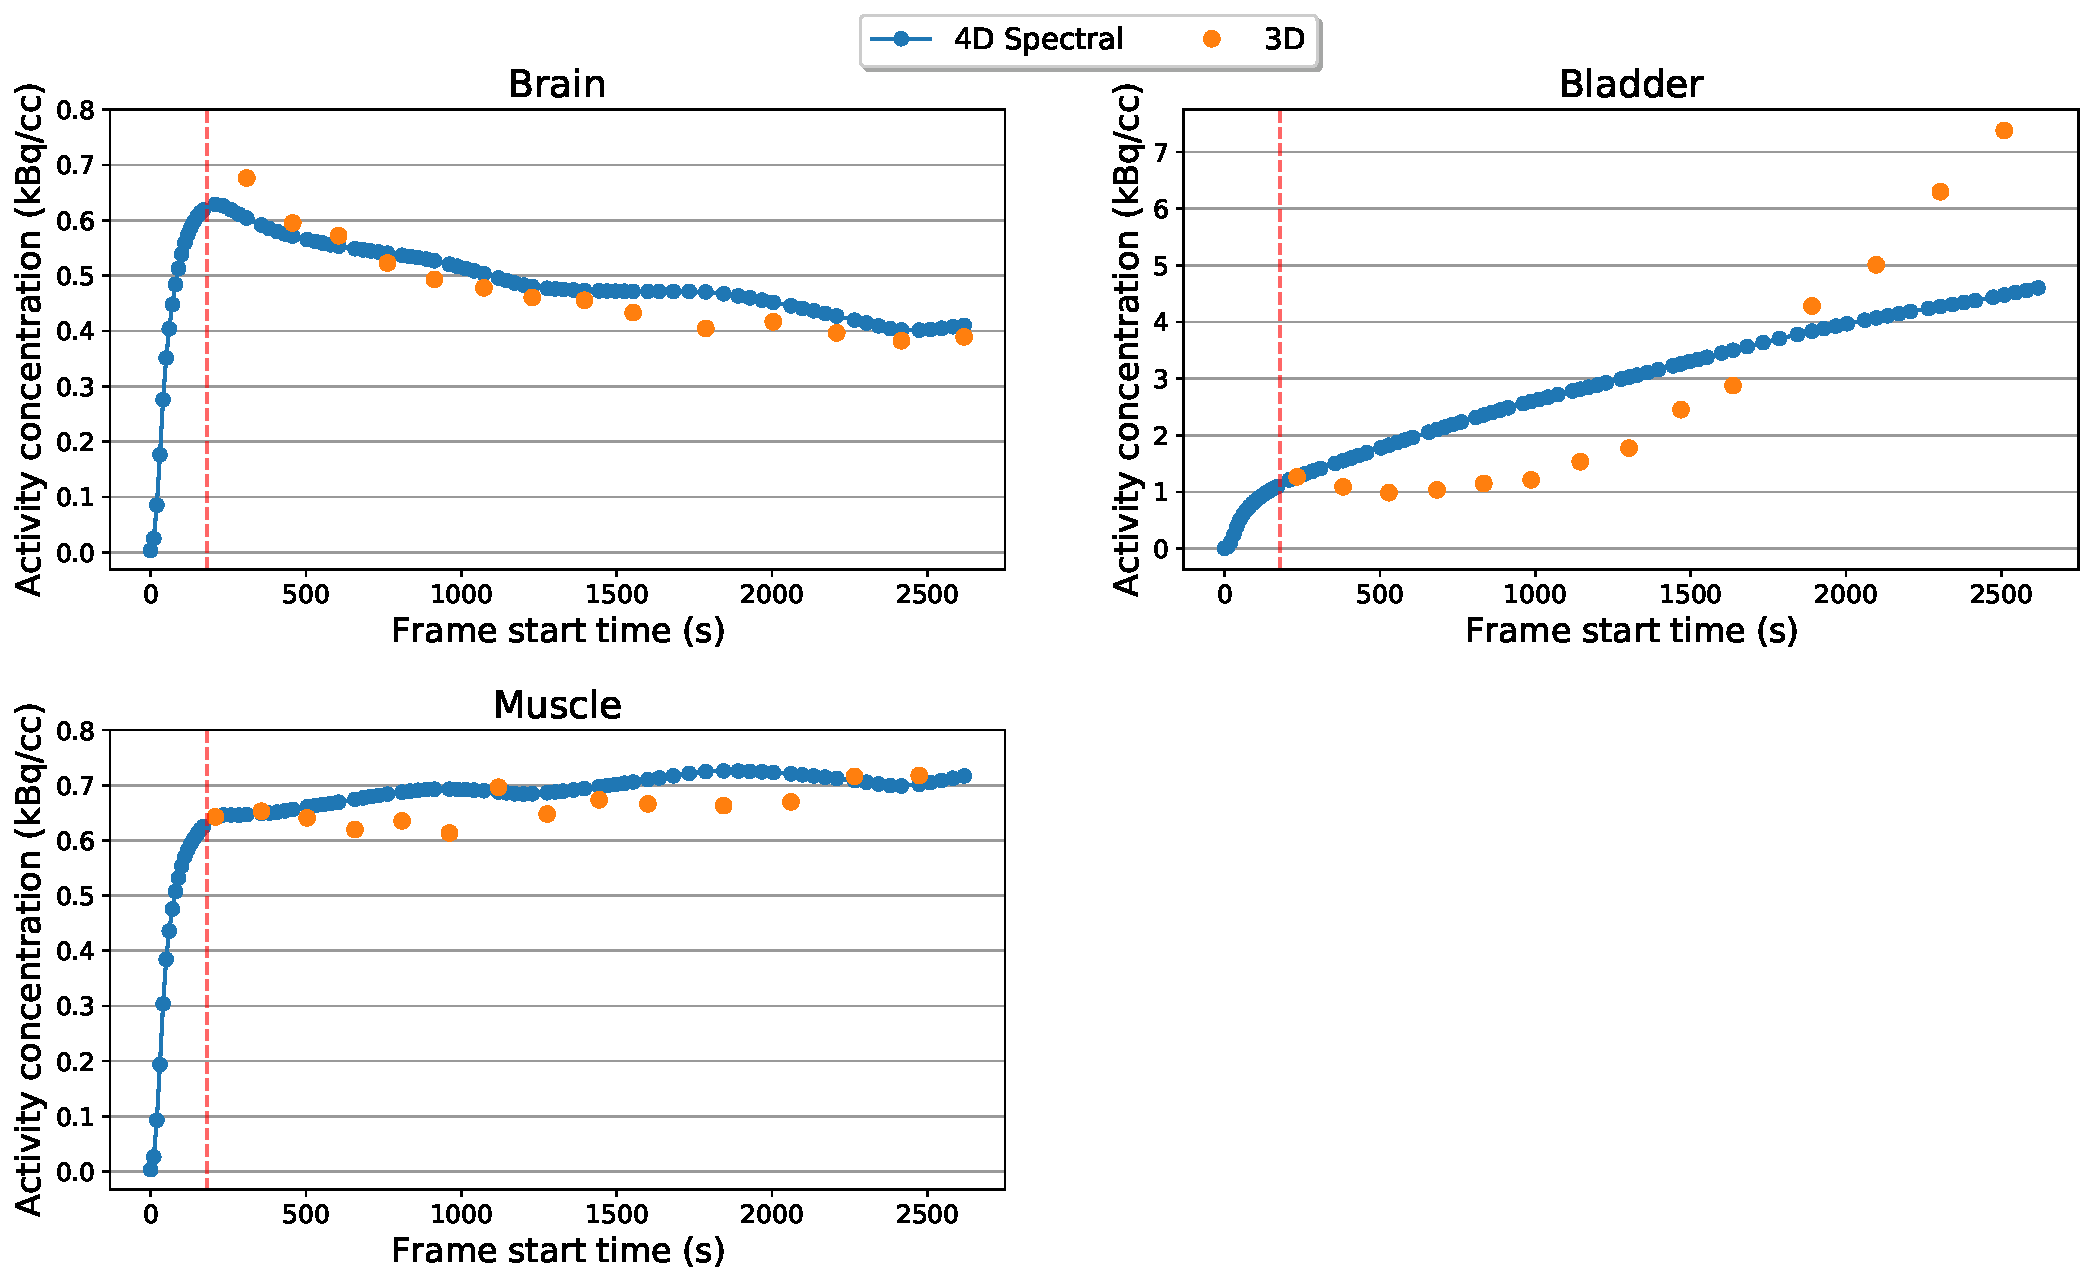
\includegraphics[scale=0.5,angle=0]{3_Results/3_3_DWB_Reconstruction/figures/3_3_IsotoPK_CTRL_DWB_3D_vs_4D_peripheral.pdf}
\caption{VOI mean time activity curves for 3D and 4D spectral reconstruction. VOI regions shown which are covered only by the DWB acquisition, whose start time is designated with a vertical dotted line.}
\label{fig_3_3:IsotoPK_CTRL_DWB_4D_vs_3D_Peripheral}
\end{figure} 

\subsection{Comparison of 4D Spectral reconstruction on DWB data, with and without the use of DSB data}
A comparison between 4D spectral reconstruction with and without the use of the initial DSB data is made in figure~\ref{fig_3_3:IsotoPK_CTRL_DWB_4D_vs_3D_Peripheral} for VOIs covered by both acquisitions. These show a good agreement of the two spectral reconstruction, with a consistent error in the early frame estimations of the reconstruction without use of DSB data, that is relatively small compared to the mean activity of each VOI (maximum of 12.7\% error seen in Spleen VOI). A very good agreement is seen on the liver between the two reconstructions.

The extrapolation of the fitted spectral model from DWB data alone can be made for the early frames. These show a sharp drop of the fitted TACs, indicating the inadequacy of the used data for extrapolation of the fast early frame behaviour. 

\begin{figure} [h!]
\centering
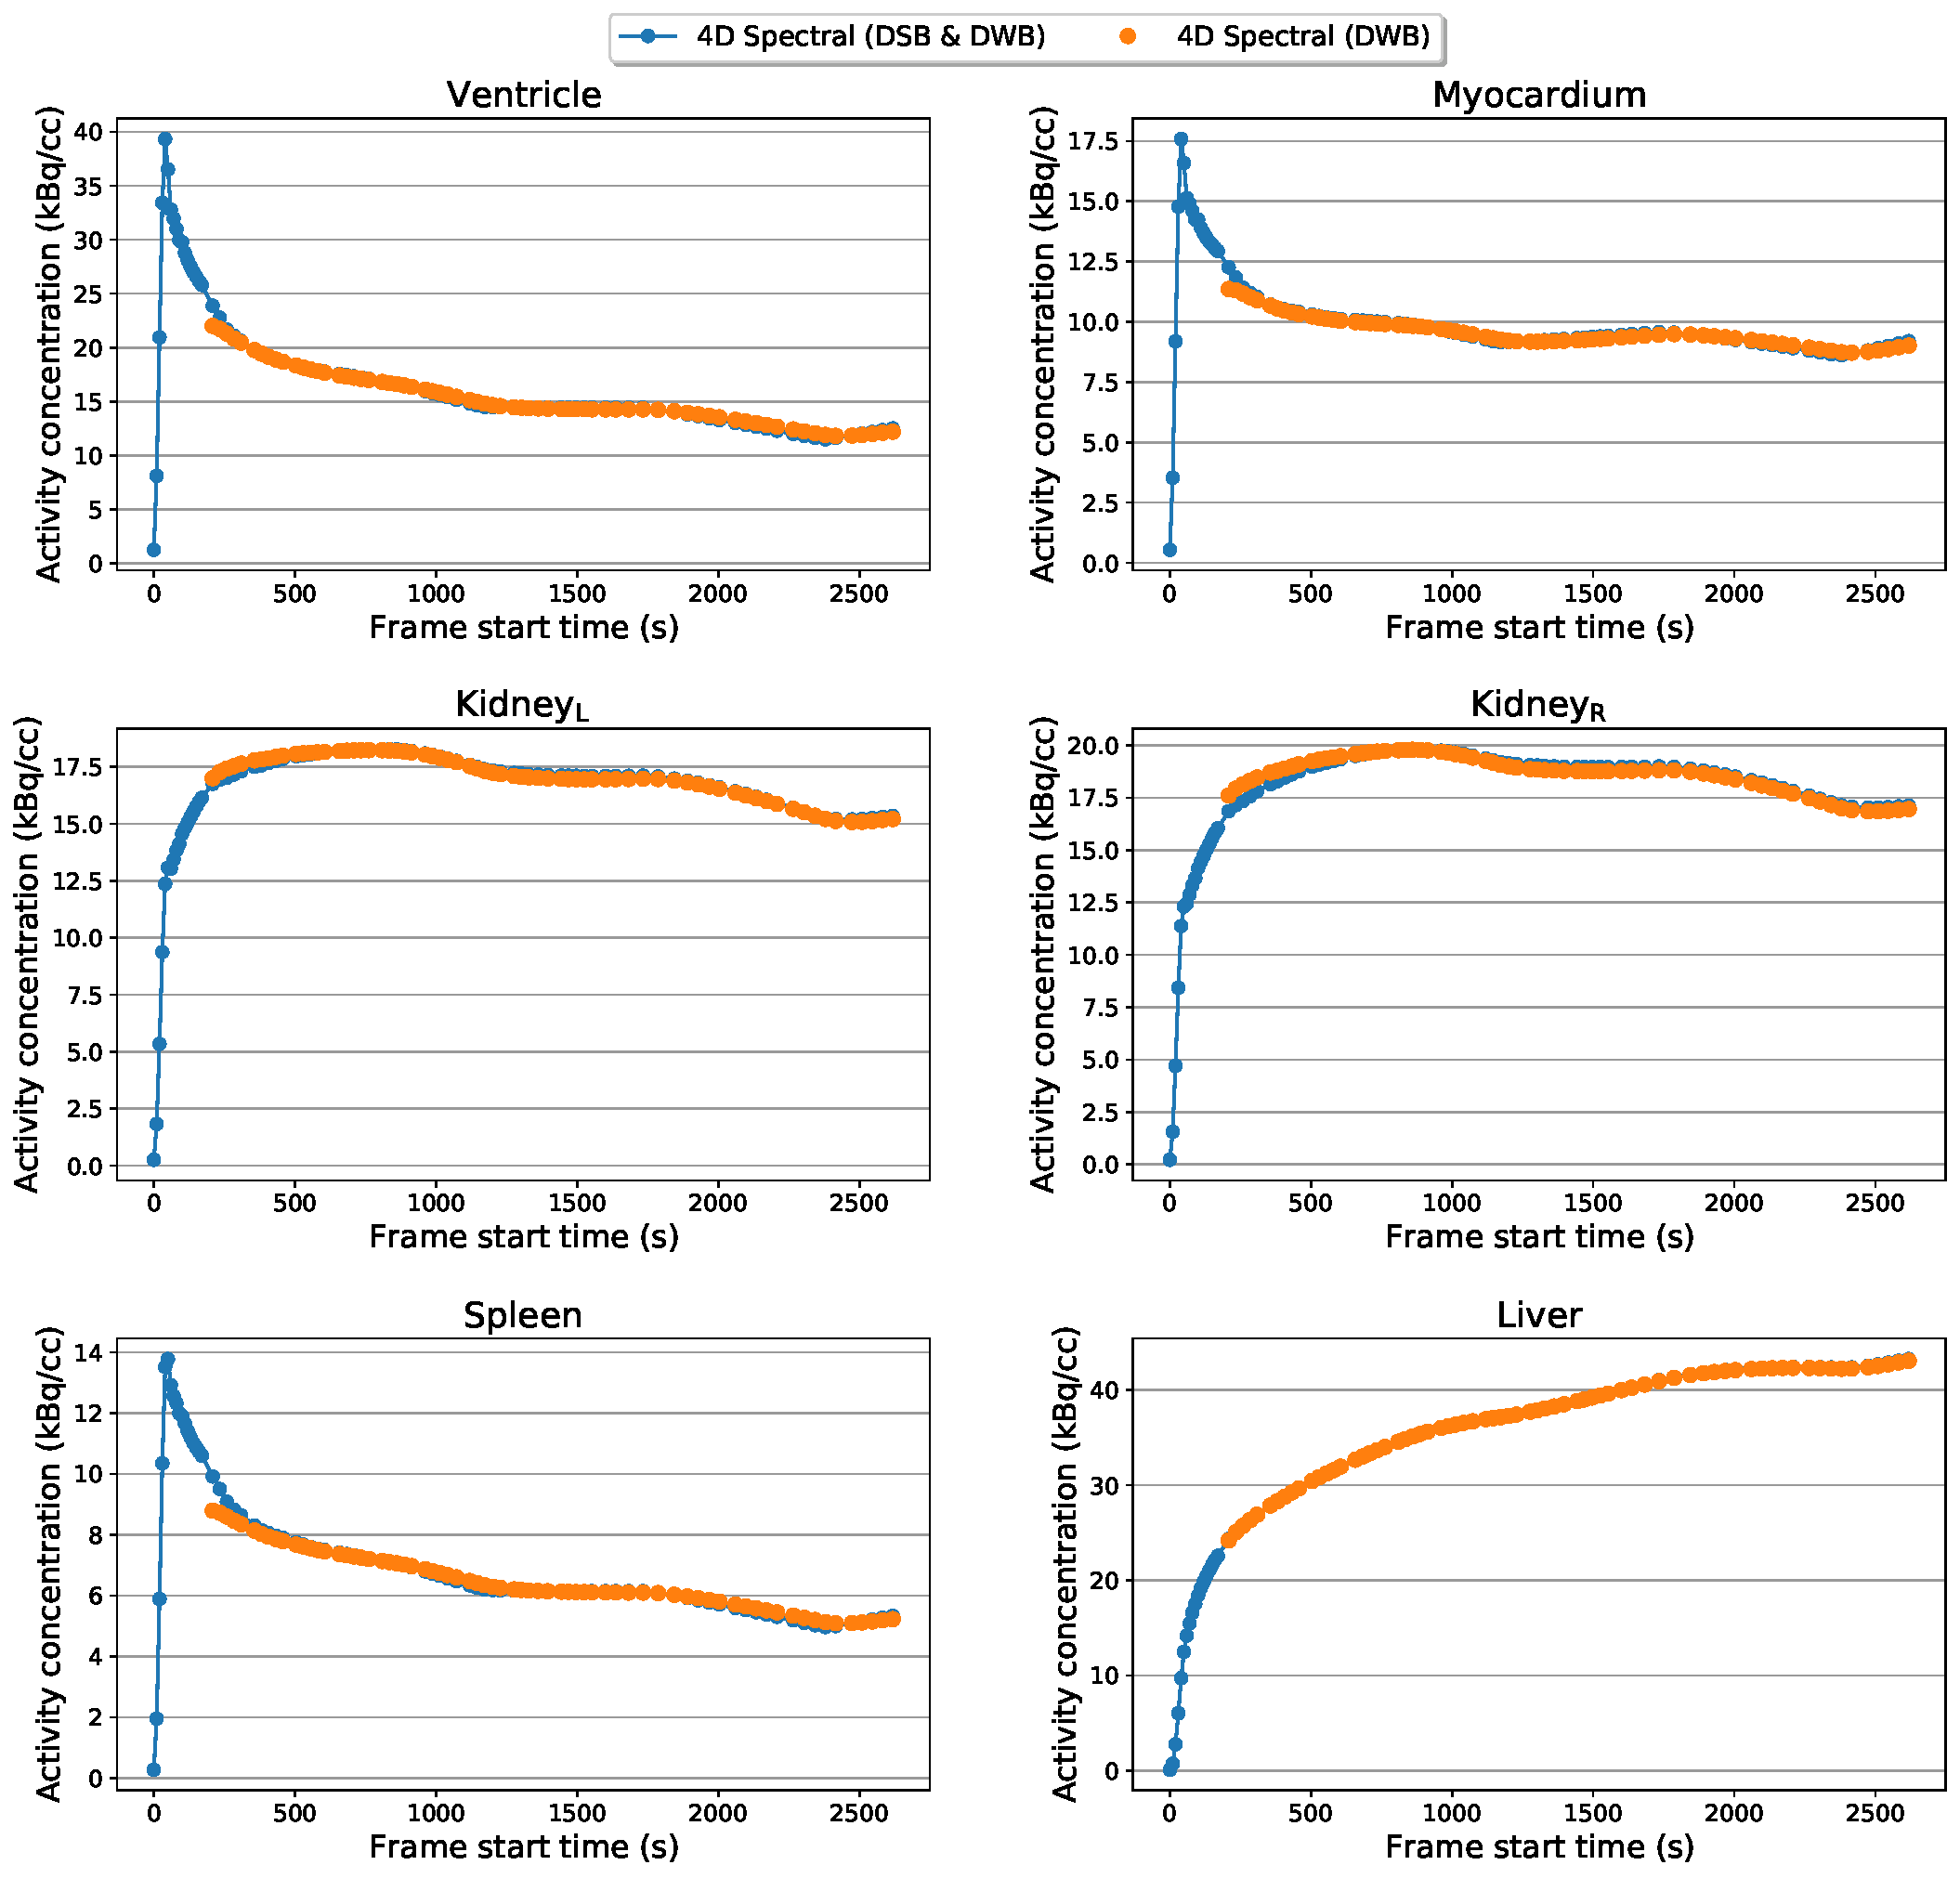
\includegraphics[scale=0.5,angle=0]{3_Results/3_3_DWB_Reconstruction/figures/3_3_IsotoPK_CTRL_DWB_4D_vs_4D_central.pdf}
\caption{VOI mean time activity curves for 4D spectral reconstructions, with and without the use of DSB data. VOI regions shown are included in both DSB and DWB acquisitions.}
\label{fig_3_3:IsotoPK_CTRL_DWB_4D_vs_3D_Peripheral}
\end{figure} 

\subsection{Direct WB parametric image estimation from 4D Spectral reconstructions}
Using the set of equations~\ref{eqn:AllSpectralEqns} and specifically the equation for the derivation of $K_1$, the parametric maps of $K_1^{*}$ were produced by summation of basis $(\phi_0-\phi_{M-1})$. Similar to the simulation study before, the blood fraction correction term $(1-\phi_M)$ was neglected in favour of avoiding voxel-to-voxel division and induction of excessive image noise. The result parametric maps for both \textit{CTRL} and \textit{RIF} scans are shown in figure~\ref{fig_3_3:IsotoPK_K1_MIP} and figure, as a \gls{mip} in the coronal plane and as a single coronal slice showing the the liver, kidneys and the spleen.
Mean VOI $K_1^{*}$ values were calculated from the parametric images and corrected with the mean $\phi_M$ value to calculate the VOI $K_1$ values shown in figure~\ref{fig_3_3:IsotoPK_K1_drop}. 

\begin{figure} [h!]
\centering
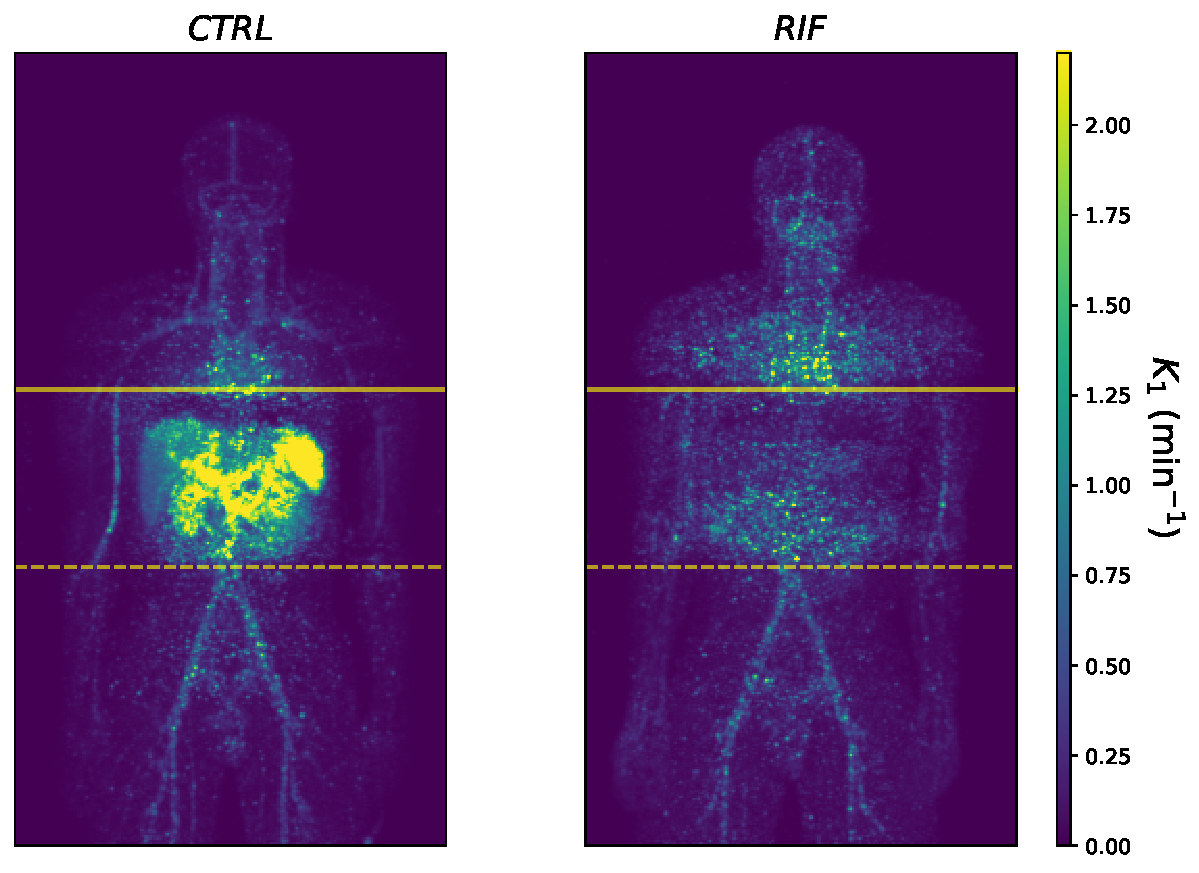
\includegraphics[scale=0.5,angle=0]{3_Results/3_3_DWB_Reconstruction/figures/3_3_IsotoPK_K1_MIPs.pdf}
\caption{$K_1$ MIP images from the 4D spectral reconstruction using both DSB and DWB acquisitions, shown for the \textit{CTRL} and \textit{RIF} scan.}
\label{fig_3_3:IsotoPK_K1_MIP}
\end{figure} 

\begin{figure} [h!]
\centering
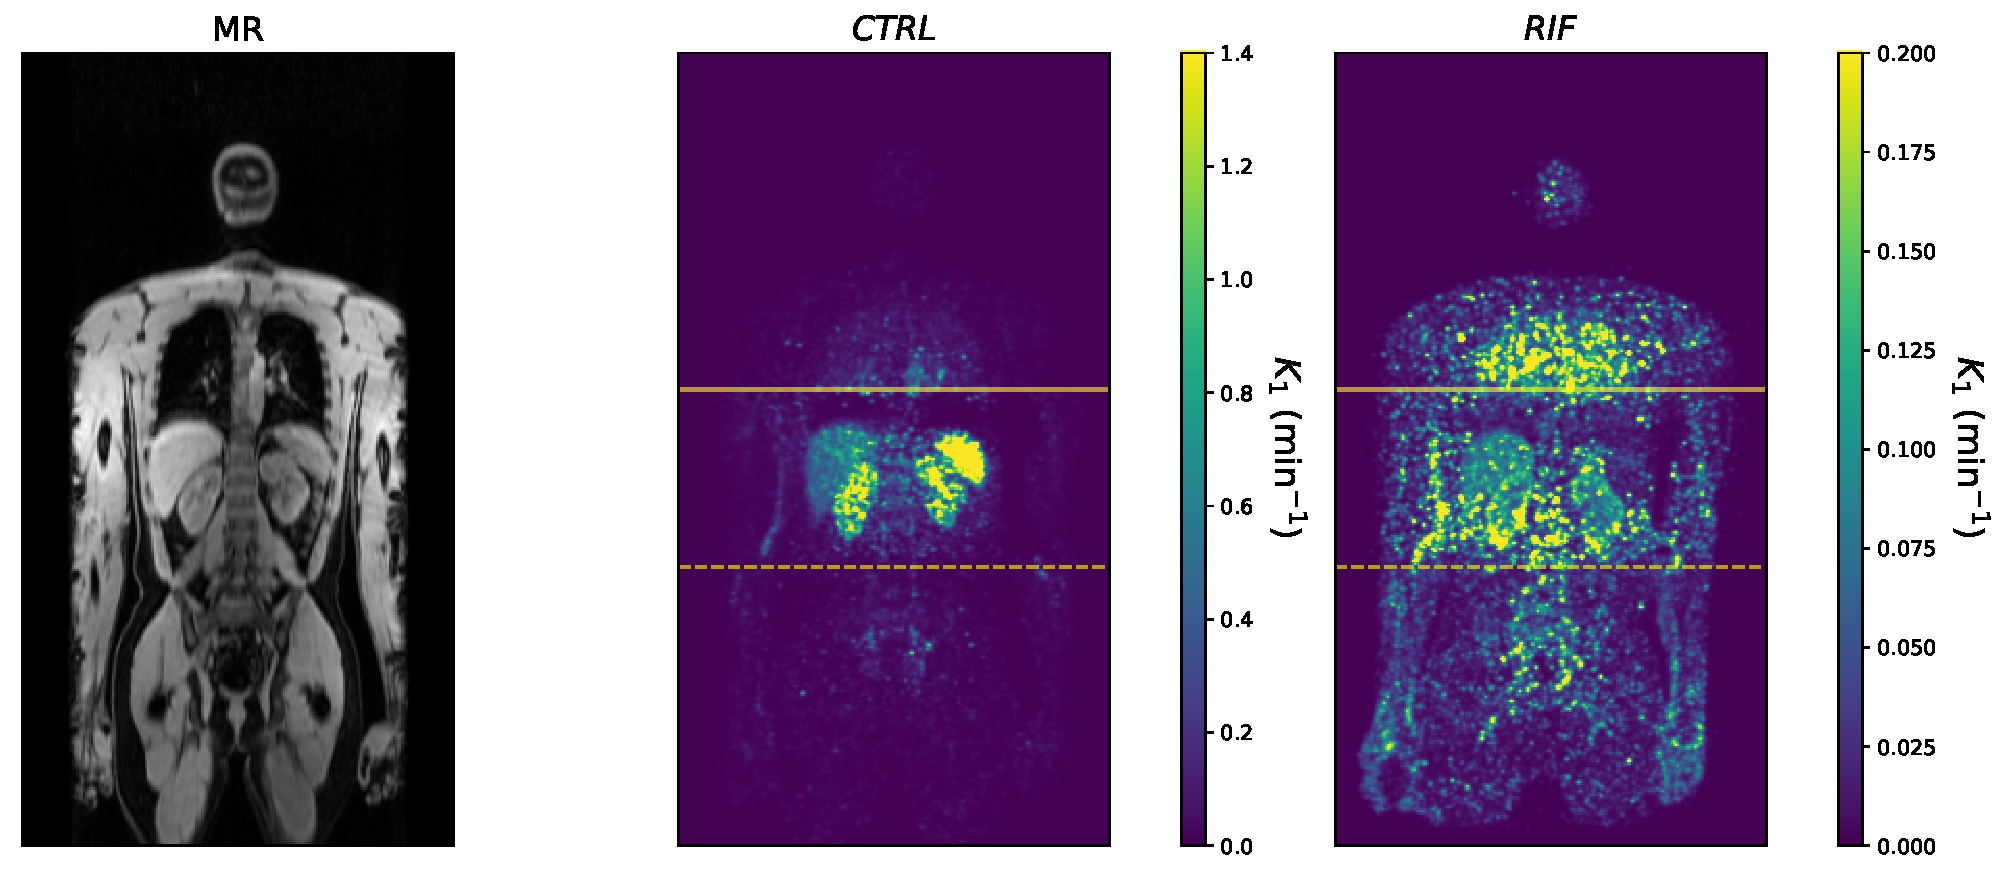
\includegraphics[scale=0.5,angle=0]{3_Results/3_3_DWB_Reconstruction/figures/3_3_IsotoPK_K1_SingleSlice.pdf}
\caption{$K_1$ values as estimated from the 4D spectral reconstruction for VOI regions included in both DSB and DWB acquisitions , shown for the \textit{CTRL} and \textit{RIF} scan}
\label{fig_3_3:IsotoPK_K1_SingleSlice}
\end{figure} 

\begin{figure} [h!]
\centering
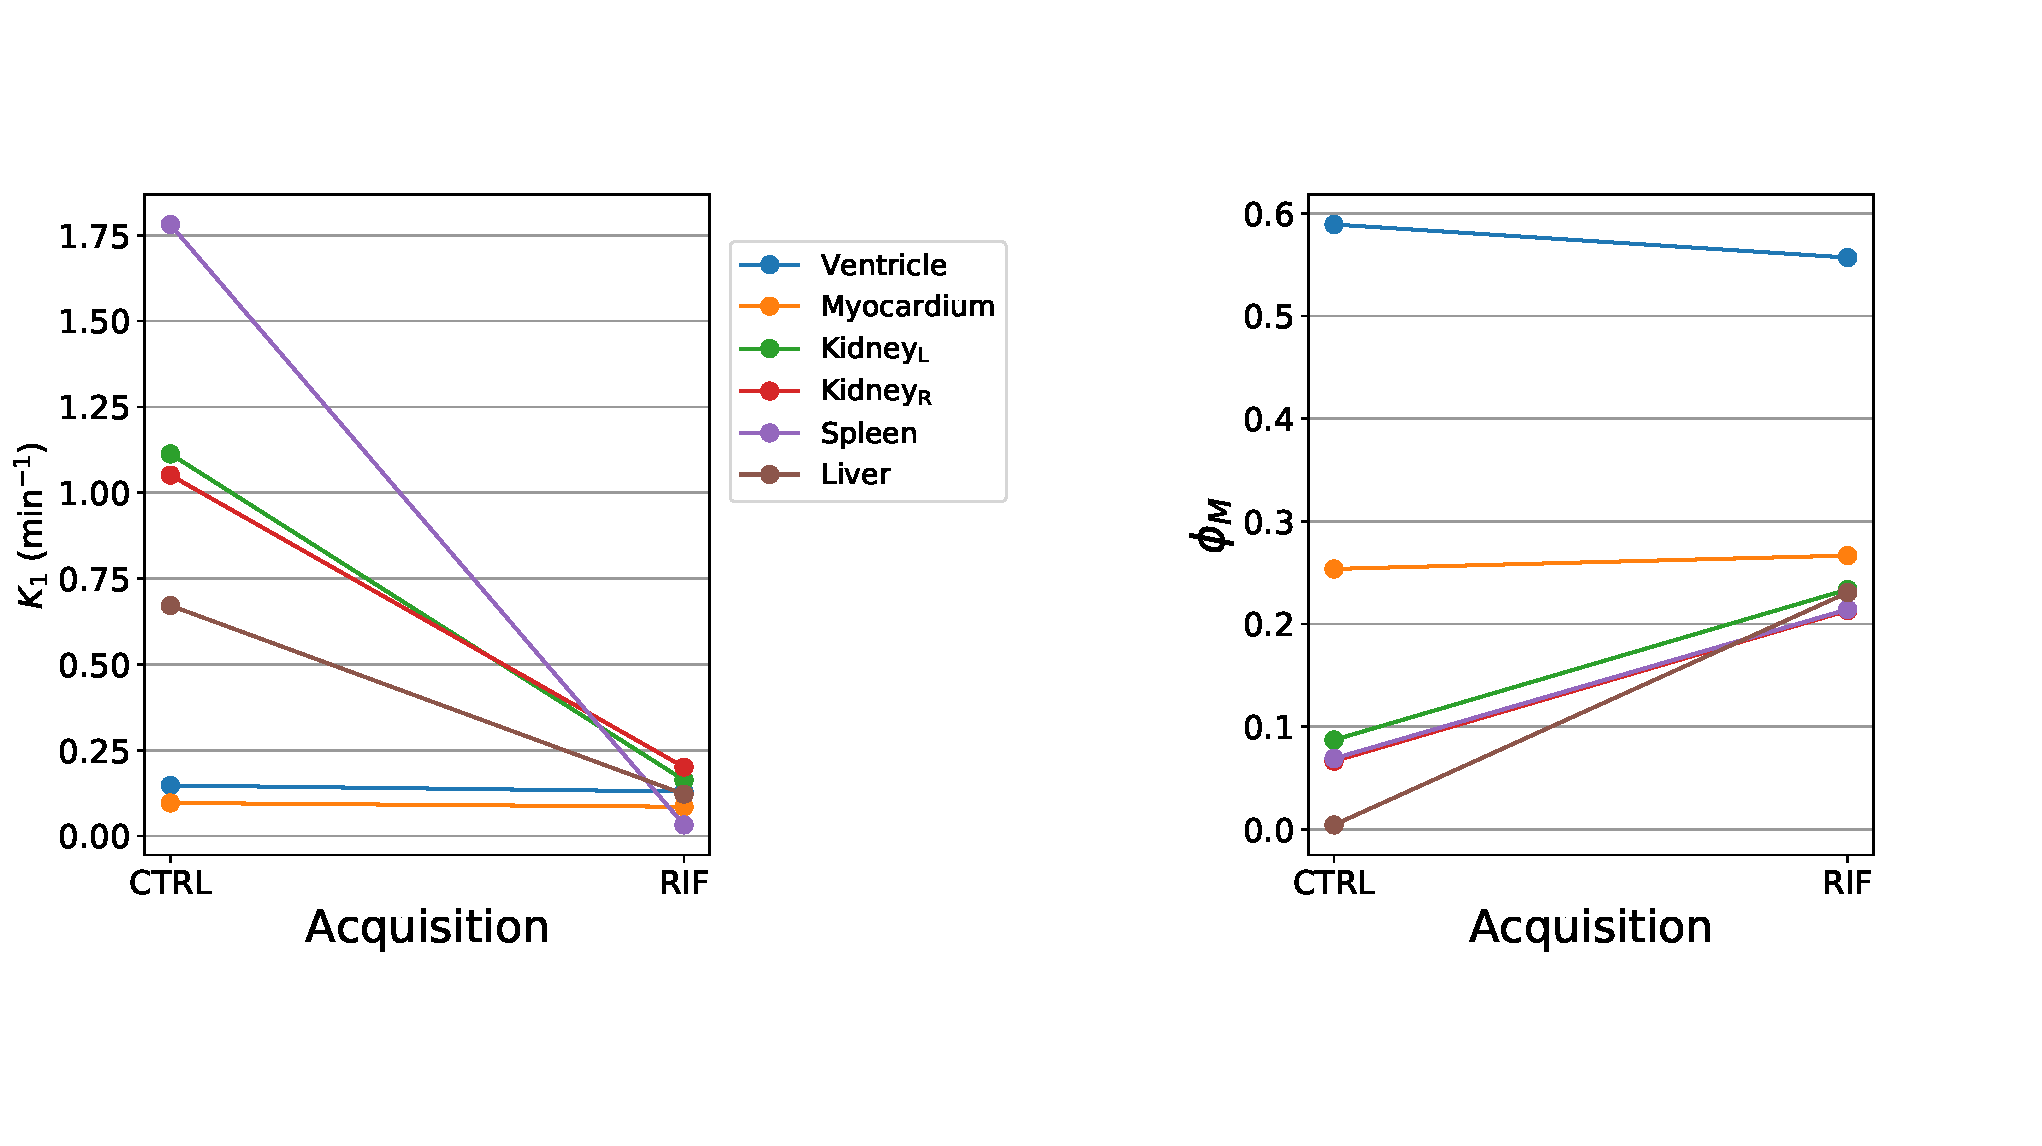
\includegraphics[scale=0.5,angle=0]{3_Results/3_3_DWB_Reconstruction/figures/K1_VB_drop.pdf}
\caption{$K_1$ values as estimated from the 4D spectral reconstruction for VOI regions included in both DSB and DWB acquisitions , shown for the \textit{CTRL} and \textit{RIF} scan}
\label{fig_3_3:IsotoPK_K1_drop}
\end{figure} 

\subsubsection{Liver dual-input blood toy simulation}
The effectiveness of the spectral model in assessing relative differences of $K_1$ while not accounting for the explicit dual-input function of this particular organ was tested with a simulation. The aim was to get an understanding of the behaviour of the model, when fitted using only the arterial input function, and to assess if relative differences such as the ones showed above between the \textit{CTRL} and \textit{RIF} scans can translate to relative differences of true underlying $K_1$ changes. 

\subsection{Fit errors and residual modelling}
\label{sub_section:residuals}


\newpage
\newpage
\newpage
\section{Discussion}

We have presented a framework for direct multi-bed reconstruction of DWB datasets, for individual frame reconstruction as well as dynamic reconstructions. The flexibility offered by this framework and by the CASToR reconstruction platform allows for the use of the DSB data that are commonly acquired prior to DWB acquisition, in the same reconstruction loop. We have shown how the framework can be extended for use with nested optimization for dynamic reconstruction.

We performed an inconclusive evaluation study with the NHP dataset by splitting the acquired data into 10 replicates, to evaluate differences between the post-reconstruction overlapping of parametric image and direct multi-bed DWB reconstruction of parametric images. But results were inconclusive and showed the need for a detailed simulation study to assess differences in terms of bias and noise properties of the overlapping regions. 

Talk about need of comparison on current state of the art practices for S\&S mutli-bed DWB, by overlapping parametric images, to the proposed method. Talk about how this was 
